\documentclass[a4paper,11pt]{article}
\pdfoutput=1

\usepackage{jheppub}

%\usepackage[T1]{fontenc} % if needed
\usepackage{amsmath,amssymb,graphicx}
\usepackage{subfigure}
\usepackage{multirow}
\usepackage{dcolumn}
\usepackage{color,url}
\usepackage{colordvi}
\usepackage{bm}
\usepackage{siunitx}
\usepackage{slashed}
\usepackage{natbib}
\usepackage{hyperref}
\usepackage{makecell}
\usepackage{pbox}
%\usepackage{fourier} 
\usepackage{array}
\newcommand{\bea}{\begin{eqnarray}}
\newcommand{\eea}{\end{eqnarray}}
\newcommand{\beq}{\begin{eqnarray}}
\newcommand{\eeq}{\end{eqnarray}} 
\newcommand{\CL}{{\cal L}}
\newcommand{\power}[2]{{#1}^{#2}}
\newcommand{\ud}{\mathrm{d}}
\newcommand{\arxiv}[1]{\href{http://arxiv.org/abs/#1}{\color{blue}{#1}}}

\newcommand{\mgamc}{Madgraph5\_aMC@NLO}
\newcommand{\whizard}{WHIZARD}

\newcommand{\xznote}[1]{\textbf{[X.Z.:}\textit{\textcolor{blue}{\Large #1}}\textbf{]}}

\newcommand{\bra}[1]{\langle#1|}
\newcommand{\ket}[1]{|#1\rangle}

\newcommand{\gwa}[1]{g_{W,a#1}}
\newcommand{\gwb}[1]{g_{W,b#1}}
\newcommand{\gwc}[1]{g_{W,c#1}}
\newcommand{\gza}[1]{g_{Z,a#1}}
\newcommand{\gzb}[1]{g_{Z,b#1}}
\newcommand{\gaa}[1]{g_{A,a#1}}
\newcommand{\gab}[1]{g_{A,b#1}}
\newcommand{\gzc}[1]{g_{Z,c#1}}
\newcommand{\gva}[1]{g_{V,a#1}}
\newcommand{\gvb}[1]{g_{V,b#1}}
\newcommand{\gxa}[1]{g_{X,a#1}}
\newcommand{\gxb}[1]{g_{X,b#1}}

\def\missE{\slashed E} % missing E

\title{\boldmath Measuring B anomalies by $\mu^+\mu^-\to tc$ at future lepton colliders}

%\author[a]{Wolfgang Kilian}
\author[a]{Sichun Sun}
\author[b,c]{Qi-Shu Yan}
\author[d]{Xiaoran Zhao}
\author[c,e]{Zhijie Zhao}

%\affiliation[a]{Department of Physics, University of Siegen, 57072 Siegen, Germany}
\affiliation[a]{School of Physics, Beijing Institute of Technology, Beijing, 100081, China}
\affiliation[b]{School of Physics Sciences, University of Chinese Academy of Sciences, Beijing 100039, China}
\affiliation[c]{Center for Future High Energy Physics, Institute of High Energy Physics, Chinese Academy of Sciences, Beijing 100039, China}
\affiliation[d]{Dipartimento di Matematica e Fisica, Universit{\`a} di Roma Tre and \\
INFN, sezione di Roma Tre, I-00146 Rome, Italy}
\affiliation[e]{DESY, Notkestr. 85, 22607 Hamburg, Germany}


%\emailAdd{kilian@physik.uni-siegen.de}
\emailAdd{sichunssun@gmail.com}
\emailAdd{yanqishu@ucas.ac.cn}
\emailAdd{xiaoran.zhao@uniroma3.it}
\emailAdd{zhijie.zhao@desy.de}

\preprint{}


\abstract{
Motivated by B anomalies, we study the matching procedure of operators $O_9, O_{10}$ in the low energy effective Hamiltonian and operators in the Standard Model effective theory (SMEFT). It is noticed that there are more related operators in the SMEFT whose coefficients can not be determined only from the low energy data from the B anomalies. We demonstrate how to determine these coefficients with some new physics models, like $Z^\prime$ model and leptoquark models, and then consider how to probe these operators of SMEFT at high energy by using the process $\mu^+\mu^-\to tc$ at future muon colliders, which can provide complementary information except for  $\mu^+ \mu^- \to b s$ on the underlying models which lead to B anomalies. We perform a Monte Carlo study (a hadron level analysis) to show how to separate the signal events from the SM background events and estimate the sensitivity to the Wilson coefficients for different models.
}

\begin{document}
\maketitle
\flushbottom


\section{Introduction}
Searching for new physics is the prime target of both the high energy frontier and high precision frontier.
In the rare decays of B mesons, there exist long-standing discrepancies between the Standard Model predictions and experimental measurements, with a hint of non-lepton flavor universality(LFU), especially in the muon-related final states. These B-anomalies are observed in a $B \rightarrow K \mu^+ \mu^-$,  $B_s \rightarrow \phi  \mu ^+ \mu^-, B_s \rightarrow  \mu ^+ \mu^-$ and angular distribution of  $B \rightarrow K^* \mu ^+ \mu^-$\cite{LHCb:2021awg,LHCb:2021vsc,LHCb:2017rmj,ATLAS:2018cur,CMS:2019bbr}. For the LFU violation, it has been observed by LHCb\cite{LHCb:2021trn,LHCb:2019hip,LHCb:2017avl,LHCb:2015svh,LHCb:2020lmf,LHCb:2020gog} in the ratio 

\begin{eqnarray}
R_K = \frac{BR(B \rightarrow K \mu^+ \mu^-)}{BR(B \rightarrow K e^+ e^-)}, R_{K^*} = \frac{BR(B \rightarrow K^* \mu^+ \mu^-)}{BR(B \rightarrow K^* e^+ e^-)}
\end{eqnarray}

Although large hadronic uncertainties can enter in some of these absolute branching fractions and angular observables for the Standard Model predictions, $R_K, R_{K^*}, B_s \rightarrow  \mu ^+ \mu^- $ are considered relatively theoretically clean. The deviation in those measurements might lead to indirect evidence for new physics \cite{Hiller:2014ula, Altmannshofer:2017fio, Altmannshofer:2014rta,Geng:2017svp,Ciuchini:2019usw,Datta:2019zca,Aebischer:2019mlg,Ciuchini:2020gvn,Jager:2017gal}. While that measurement provides derivation from SM prediction,
the exact mechanics behind those anomalies are still unknown,
and low-energy measurement cannot fully reveal the nature behind that.

On the other hand, by scattering high-energy particles,
collider experiments provide unique opportunities to access underlying UV theories.
Among various current and future colliders\cite{Shiltsev:2019rfl},
a multi-TeV muon collider\cite{Aime:2022flm,MuonCollider:2022xlm} is ideal for such studies.
Being fundamental particles, the entire energy of incoming muons is available to produce short-distance scattering rather than being spread among partons of hadrons,
and thus a 14 TeV muon collider can be as effective as a 100 TeV proton-proton collider\cite{Delahaye:2019omf}.
Such high energy reach strongly benefits searching new heavy particles, such as minimal dark matter models\cite{Han:2020uak,Bottaro:2021snn},
as well as indirect measurement at high energies\cite{Buttazzo:2020uzc}.
Moreover, vector boson fusion processes are found to be important at muon colliders\cite{Costantini:2020stv},
and enable access to difficult parameters such as the Higgs quartic self-coupling\cite{Chiesa:2020awd}.
More importantly, muon colliders have a special feature: the initial states are muons, directly related to those low-energy anomalies. The muon $g-2$ anomaly can be probed directly at muon colliders\cite{Buttazzo:2020ibd}.
In the context of muon $g-2$ anomaly, studies have been performed on testing it under the SMEFT formalism\cite{Buttazzo:2020ibd}, and model-exhaustive analysis\cite{Buttazzo:2020ibd,Capdevilla:2020qel,Capdevilla:2021rwo,Capdevilla:2021kcf}.
%The future collider proposals include the linear or circular case $e^+e^-$ colliders\cite{} and circular pp coliders \cite{}, and especially relevant here: high-energy muon colliders \cite{}.  Muon colliders can reach high energies with large mass suppression of synchroton radiation comparing to $e^+e^-$ colliders and higher precision with cleaner final states comparing to pp colliders. Although the short life time of muon causes some technical challenges, there are a series of recent progresses\cite{}.

 The multi-TeV reach and better precision advantages of muon colliders, make it a perfect place to probe muon-related B anomalies in low energy. There are already proposals studying $\mu^+\mu^-\to b\bar{s}$ or $\bar{b}s$ at multi TeV scale to discuss the impact of low energy B-anomalies impact \cite{Altmannshofer:2022xri,Huang:2021nkl}. At the current stage, B-anomalies can be nicely parameterized  by effective four-fermion operators at the B-physics scale ($\mu= 4.8$ GeV):
 \begin{eqnarray}
   O_9 &=& (\bar{s}\gamma_\mu P_L b)(\bar{\ell}\gamma^{\mu}\ell),  \\
   O_{10} &=& (\bar{s}\gamma_\mu P_L b)(\bar{\ell}\gamma^{\mu}\gamma_5\ell),
\end{eqnarray}
For the new physics effects described by operators $O_9$ and $O_{10}$, when we go above the weak scale ($\mu=M_Z$ for instance), the Wilson coefficients of such two operators depend on the specific models (e.g. leptoquark, scalars,$Z'$,etc). 

In this work, we adopt the same assumption that the new physics scale is around $\mu=35$ TeV and it is challenging to discover the new physics signature at the LHC. We also assume that these new physics above the weak scale ($\mu=M_Z$) can be described by the framework of the standard model effective field theory (SMEFT). Under appropriate assumptions, it is noteworthy that there is at least one more operator needed in order to match the SMEFT to low energy operators $O_9$ and $O_{10}$. These three operators in the SMEFT are given in Eqs. (2.12-2.14). Different new physics models can lead to different matching conditions across the weak scale.

Different from the proposal presented in \cite{Altmannshofer:2022xri}, where the polarization of muon beams and charge tagging of jets in the final state is assumed, in this work, in order to reveal the nature of new physics which leads to the B anomalies, we propose to measure the process $\mu^+\mu^-\to tc$ (here $tc$ denotes both $t \bar{c}$ and $\bar{t} c$). This study can provide complementary information to the processes $\mu^+\mu^-\to b \bar{s}$ ($\bar{b} s$). The four fermion operators for $\mu^+\mu^-\to tc$ naturally arise from the operator matching conditions from the low energy effective field theory to the SMEFT, since left-handed top and charm quarks form electroweak SU(2) doublets respectively as the partners of the left-handed bottom and strange quarks in SMEFT operators. The process $\mu^+\mu^-\to tc$ can also help to distinguish different new physics models, which yield different operator matching conditions. We will consider one $Z^\prime$ model and three leptoquark models. 

The leptoquark particles are predicted in the grand unification models and they can either be scalar or vector bosons. Usually, these particles are superheavy (e.g. $10^{13}$ GeV), as required by the experimental data of proton decays. Very light leptoquarks (e.g. 1 TeV or a few 10 TeV) are consistent with experimental data if their couplings to the first generation of matter fields are weak. Light leptoquarks are also predicted in the Pati-Salam model, where lepton numbers are treated as the fourth color quantum number. These light leptoquarks can be accessible even at the LHC and future collider projects. Recently, leptoquarks have attracted much attention in order to interpret the B anomalies. A comprehensive on the phenomenology of leptoquarks can be found in \cite{Dorsner:2016wpm}.

Our new findings in this work include 1)  The dominant SM background events for the process $\mu^+\mu^-\to tc$ are different from the background of the process $\mu^+\mu^-\to bs$. Due to the highly boosted top quark in the final states, jet substructure analysis is crucial to distinguish signal and background events. 2) In the case that there is no new resonance found in the TeV muon colliders, measurement of the process $\mu^+\mu^-\to tc$, can provide crucial information on the potential nature of the new physics which leads to the low energy B anomalies. 3) It is noticed that the final state $W^\pm jj $ can have a very large cross section (e,g. 100fb with collision energy $\sqrt{s}=10$ TeV), and such a final state is mainly from the weak final state radiation processes. Suppressing the weak final state radiation might be important for signal findings.

This paper is organized as given below. In section II, we demonstrate the relations between the Wilsonian coefficients of the low-energy effective Hamiltonian and those of the SMEFT. In section III, we present the values of Wilsonian coefficients of the SMEFT derived from different new physics models. These new physics models can accommodate the explanation of B anomalies. In section IV, we perform a Monte Carlo simulation to explore the sensitivity of future muon colliders to these new physics scenarios. We end this work with a few discussions and conclusions. In Appendix, we present the renormalization group equations of Wilsonian coefficients in the SMEFT and effective Hamiltonian, respectively. 


%\section{Motivations for studying B-anomalies in $\mu^+\mu^-\to tc$}
\section{Matching and running of different operator bases}
\label{Sec:EFT}

 Interestingly, these anomalies can be simultaneously explained in a model-independent way with the effective four-fermion operators. 
In many B-physics studies,  new physics effects strongly prefer an effective Hamiltonian with $O_9 $ and $O_{10}$ with Wilson coefficients of dimension 6 interactions at the renormalization scale $\mu =4.8$ GeV ,
\begin{eqnarray}
  \mathcal{H}_{eff} &=& \mathcal{H}^{SM}_{eff}-\mathcal{N}\sum_{\ell=e,\mu}\sum_{i=9,10}\left(c_iO^{bs\ell\ell}_i+c^\prime_i O^{\prime bs\ell\ell}_i\right) + h.c., 
\end{eqnarray} 
where the normalization factor $\mathcal{N}$ is 
\begin{eqnarray}
  \mathcal{N} &=& \frac{4G_F}{\sqrt{2}}V_{tb}V^*_{ts}\frac{e^2}{16\pi^2}. 
\end{eqnarray}
The operators $O_9$ and $O_{10}$ are 
\begin{eqnarray}
   O^{bs\ell\ell}_9 &=& (\bar{s}\gamma_\mu P_L b)(\bar{\ell}\gamma^{\mu}\ell),  \\
   O^{bs\ell\ell}_{10} &=& (\bar{s}\gamma_\mu P_L b)(\bar{\ell}\gamma^{\mu}\gamma_5\ell),
\end{eqnarray}
where $P_L=(1-\gamma_5)/2$ is the left-handed projection operator. 
For $O^\prime_i$, $P_L$ is replaced by right-handed projection operator $P_R=(1+\gamma_5)/2$.

For the purpose of this paper, to study B-anomalies related operator $O_9$ and $O_{10}$ defined in the low energy B physics scale in higher colliding energy scale, we need to treat the running and matching of the operators carefully. 
Especially the subtleties that arise when the energy runs across the weak scale. Our study finds that in the energy scale above the weak scale, the impact of $O_9$ and $O_{10}$ operators needs to be reparametrized by three different operators, rather than two, in the so-called Warsaw basis, known as the Standard model effective theory (SMEFT). Here we introduce different bases and coefficient matching as below. 

 At the scale below the weak scale, potential new physics effects are described by a low energy effective field theory (LEFT).  
The LEFT Lagrangian with dimension 6 operators can be written as 
\begin{eqnarray}
  \mathcal{L}_{LEFT} &=& \mathcal{L}_{QCD+QED}+ \frac{1}{v^2}\sum_{i}L_iQ_i,  \nonumber 
\end{eqnarray} 
where $L_i$ are the Wilson Coefficients of LEFT, and $v=246$ GeV is the vacuum expectation value. 

In this paper, we use the convention of Ref.~\cite{Jenkins:2017jig}. 
The most relevant operators are 
\begin{eqnarray}
  Q^{V,LL}_{ed}(p,r,s,t) &=& (\bar{e}_{Lp}\gamma^\mu e_{Lr})(\bar{d}_{Ls}\gamma_\mu d_{Lt}),  \label{QVLLed} \\
  Q^{V,LR}_{de}(p,r,s,t) &=& (\bar{d}_{Lp}\gamma^\mu d_{Lr})(\bar{e}_{Rs}\gamma_\mu e_{Rt}),  \label{QVLRde}
\end{eqnarray}
where $p,r,s,t$ are generation indices of quark or lepton. 
Since the EW symmetry is broken, here $e$ and $d$ are the lepton field and down-type quark field. 
$L$ and $R$ are the chiral indices of fermions. 



One can derive the relations between $Q_i$ and $O_i$ easily:
\begin{eqnarray}
  Q^{V,LL}_{ed} &=& \frac{1}{2}\left(O_9-O_{10}\right),  \\
  Q^{V,LR}_{de} &=& \frac{1}{2}\left(O_9+O_{10}\right).   
\end{eqnarray}
So we have 
\begin{eqnarray}
  L^{V,LL}_{ed} &=& \frac{\mathcal{N}v^2}{2}(c_9-c_{10}),  \\
  L^{V,LR}_{de} &=& \frac{\mathcal{N}v^2}{2}(c_9+c_{10}). 
\end{eqnarray}
The constraints of $c_9$ and $c_{10}$ can be found in Ref.~\cite{Altmannshofer:2021qrr}.

Assuming the new physics appears at a scale above the weak scale $\Lambda$, 
the SMEFT Lagrangian with dimension 6 operators ($\mathcal{O}_i$) is defined as
\begin{eqnarray}
  \mathcal{L}_{SMEFT} &=& \mathcal{L}_{SM} + \frac{1}{\Lambda^2}\sum_{i}C_i\mathcal{O}_i,  
\end{eqnarray}
where $C_i$ are called Wilson Coefficients.

A complete set of non-redundant dimension 6 operators has been derived in Ref.~\cite{Grzadkowski:2010es}, so-called Warsaw basis. 
The most relevant operators in this paper are
\begin{eqnarray}
   \mathcal{O}^{(1)}_{lq}(p,r,s,t) &=& (\bar{l}_p\gamma^\mu l_r)(\bar{q}_s\gamma_\mu q_{t}),  \label{O1lq} \\ 
   \mathcal{O}^{(3)}_{lq}(p,r,s,t) &=& (\bar{l}_p\gamma^\mu\tau^I l_r)(\bar{q}_s\gamma_\mu\tau^I q_{t}),  \label{O3lq} \\ 
   \mathcal{O}_{qe}(p,r,s,t) &=& (\bar{q}_p\gamma^\mu q_r)(\bar{e}_s\gamma_\mu e_t), \label{Oqe}
\end{eqnarray}
where $q$, $l$, $e$ are the left-handed quark doublet, left-handed lepton doublet, and right-handed lepton singlet, respectively. 
$p,r,s,t$ are generation indices of quark or lepton.

When the electroweak symmetry breaking occurs, the SM heavy particles (top, Higgs,  $W^\pm$,  $Z$) are integrated out, and the SMEFT should be matched to LEFT. 
The full matching conditions at the tree level have been derived by Ref.~\cite{Jenkins:2017jig}.
In this paper, we only consider the operators with flavor indices $(p,r,s,t)=(2,2,2,3)$ or $(p,r,s,t)=(2,3,2,2)$, so the matching conditions are simplified to 
\begin{eqnarray}
    L^{V,LL}_{ed}(2,2,2,3) &=& \frac{v^2}{\Lambda^2}\left[C^{(1)}_{lq}(2,2,2,3)+C^{(3)}_{lq}(2,2,2,3)\right],  \label{match:VLLed}\\
    L^{V,LR}_{de}(2,3,2,2)&=& \frac{v^2}{\Lambda^2}C_{qe}(2,3,2,2). \label{match:VLRde}
\end{eqnarray}
% \bigskip
The related renormalization group equations for the SMEFT and LEFT can be found in Appendix \ref{smeftrge} and Appendix \ref{leftrge}, respectively.

\begin{center}
\begin{table}
  \begin{center}
  \begin{tabular}{|c|c|c|c|c|}
  \hline
  &      $c_9=-0.73$    &     $c_9=0.00$      &       $C_9=0.05$     &       $c_9=-0.39$       \\
  &      $ c_{10}=0.00$    &     $c_{10}=0.54$      &       $c_9=c_{10}$     &       $c_9=-c_{10}$       \\
  \hline  
                   $L^{V,LL}_{ed}(m_B)$ &   $-1.73\times 10^{-5}$   &   $-1.28\times 10^{-5}$   &  $0.00$    &    $-1.85\times 10^{-5}$    \\
                   $L^{V,LL}_{ed}(m_Z)$  &   $-1.75\times 10^{-5}$  &   $-1.29\times 10^{-5}$   &  $5.65\times 10^{-9}$  &  $-1.86\times 10^{-5}$  \\
                   $(C^{(1)}_{lq}+C^{(3)}_{lq})(m_Z)$  &   $-2.90\times 10^{-2}$  &    $-2.10\times 10^{-2}$   &   $9.34\times 10^{-6}$  &  $-3.10 \times 10^{-2}$  \\
                   $(C^{(1)}_{lq}+C^{(3)}_{lq})(\Lambda)$  &  $-3.00 \times 10^{-2}$   &  $-2.30\times 10^{-2}$  &  $2.05\times 10^{-5}$  &  $-3.20\times 10^{-2}$ \\                    
  \hline  
  $L^{V,LR}_{de}(m_B)$ &  $-1.73\times 10^{-5}$  & $1.28\times 10^{-5}$ & $2.36\times 10^{-6}$ & $0.00$ \\ 
  $L^{V,LR}_{de}(m_Z)$ & $-1.72\times 10^{-5}$  & $1.27\times 10^{-5}$ &  $2.36\times 10^{-6}$ & $-4.41\times 10^{-8}$   \\
  $C_{qe}(m_Z)$  &   $-2.80 \times 10^{-2}$   &  $2.10\times 10^{-2}$  & $3.89\times 10^{-3}$ &  $-7.28\times 10^{-5}$ \\
  $C_{qe}(\Lambda)$  &  $-2.90\times 10^{-2}$   &  $2.14\times 10^{-3}$  &   $3.99\times 10^{-3}$   &  $-2.02\times 10^{-4}$  \\
  \hline
  \end{tabular}
  \end{center}
  \caption{The coefficients $L^{V,LL}_{ed}$, $L^{V,LR}_{de}$, $C^{(1)}_{lq}+C^{(3)}_{lq}$ and $C_{qe}$ at scale $m_B=5$ GeV, $m_Z=91.19$ GeV and $\Lambda=10$ TeV are listed, with difference input of $c_9$ and $c_{10}$. Here, we assume $C^{(1)}_{lq}=3C^{(3)}_{lq}=\frac{3}{4}L^{V,LL}_{ed}\times \Lambda^2/v^2$. \label{table:LVLLed}}
\end{table}
\end{center}

\section{The Matching Conditions of New Physics}


At muon colliders, the operators we input are actually Eq.(\ref{O1lq}) to Eq. (\ref{Oqe}).
 In massless limit,\footnote{For simplicity, in this section we work under the massless limit. Nevertheless, for the numerical results discussed in later sections, full mass dependence is included} the differential cross section for $\mu^+\mu^-\to tc$ and  $\mu^+\mu^-\to bs$ are:
 \begin{align}
     \frac{\ud\sigma(\mu^+\mu^-\to X)}{\ud\cos\theta}=\frac{3s}{256\pi}|C_{LL}^{X}|^2(1+\cos\theta)^2
 \end{align}
 where
 \begin{align}
 C_{LL}^{bs}=C_{lq}^{(1)}+C_{lq}^{(3)},C_{LL}^{tc}=C_{lq}^{(1)}-C_{lq}^{(3)}
 \end{align}

Integrating over $\cos\theta$, we can obtain the inclusive cross section as:
\begin{align}
    \sigma(\mu^+\mu^-\to X)=\frac{1}{32\pi}s|C_{LL}^{X}|^2
\end{align}

In a general new physical model,
both $C_{lq}^{(1)}$ and $C_{lq}^{(3)}$ can be both non-zero,
and thus both processes $\mu^+\mu^-\to tc$ and $\mu^+\mu^-\to bs$ receives new physical contribution,
to be measured in future muon colliders.
We note that for $\mu^+\mu^-\to bs$, the corresponding Wilson coefficients $C_{LL}^{bs}$ is directly in charge of $b\to s\mu^+\mu^-$ transition in $B$-physics,
and hence constrained by those measurements.
On the other hand, $C_{LL}^{tc}$ is unconstrained.
As a general argument, the underlying new physical which induces $C_{LL}^{bs}$ or equivalently $C_{lq}^{(1)},C_{lq}^{(3)}$,
would induce also $C_{LL}^{tc}$ with size at similar order.

Therefore, we expect that the cross-section of $\mu^+\mu^-\to tc$ is comparable to $\mu^+\mu^-\to bs$,
and as we will show in Section \ref{Sec:result}, due to the presence of top quark in the final state of $\mu^+\mu^-\to tc$,
it is easier to measure than $\mu^+\mu^-\to bs$.
To be more specific, below we discuss four types of new physics models labeled as Model I-IV, 
where the relations between $C_{LL}^{tc}$ and $C_{LL}^{bs}$ are given,
and later in Section \ref{Sec:result} we will show how to distinguish them by measuring both $\mu^+\mu^-\to tc$ and $\mu^+\mu^-\to bs$.

\begin{enumerate}
    \item[Model I]   A $Z^{\prime}$ model with flavor symmetry $U(1)_{L_{\mu}-L_{\tau}}$.
        In this model, the $L_{\mu}-L_{\tau}$ is promoted into a $U(1)$ gauge symmetry,
      with a massive gauge boson $Z^{\prime}$.
    Originally it was proposed for muon $g-2$ anomaly \cite{Baek:2001kca} and neutrino mixing \cite{Ma:2001md}.
    Later it is realized that the coupling to quarks can be described by high dimensional operators, which can be generated through new heavy quarks \cite{Fox:2011qd}.
    Such interaction can induce flavor violation \cite{Altmannshofer:2014cfa}, to explain B anomaly.
    Since the effective interaction between $bs\mu\mu$($tc\mu\mu$) is mediated by an $s$-channel $Z^{\prime}$, an electroweak singlet,
    clearly we have $C_{lq}^{(3)}=0,C_{LL}^{bs}=C_{LL}^{tc}=C_{lq}^{(1)}$.
    Consequently, we have $\sigma(tc)\sim\sigma(bs)$.

    \item[Model II] A scalar triplet leptoquark $S_3$ model.
        In this model, the new physics is mediated by a heavy scalar leptoquark, which belongs to $SU(2)_L$ triplet.
        The corresponding Lagrangian can be written as \cite{Dorsner:2016wpm}
        \begin{align}
            \mathcal{L}_{NP}=\sum_{i,j}\lambda_{ij}\bar{Q}_i^c(i\tau^2)\tau^{I}L_jS_3^{I}+\textrm{h.c.}
        \end{align}
        In this model, both $C_{lq}^{(1)}$ and $C_{lq}^{(3)}$ can be generated at tree-level, which is given by \cite{Gherardi:2020det}
        \begin{align}
            [C_{lq}^{(1)}]_{prst}=&3\frac{\lambda_{sp}^{*}\lambda_{tr}}{4M^2}\\
            [C_{lq}^{(3)}]_{prst}=&\frac{\lambda_{sp}^{*}\lambda_{tr}}{4M^2}.
        \end{align}
        where $M$ is the mass of the leptoquark $S_3$.
        Therefore, we have $C_{LL}^{bs}=2C_{LL}^{tc}$,
        and $\sigma(tc)=\frac{1}{4}\sigma(bs)$

    \item[Model III] A scalar singlet leptoquark $S_1$ model.
        In this model, new physics is mediated by a heavy scalar leptoquark, which belongs to $SU(2)_{L}$ singlet.
        There are three possible hypercharge assignments,
        and we consider the case $Y=\frac{1}{3}$ here.
        The corresponding Lagrangian is
        \begin{align}
            \mathcal{L}_{NP}=\sum_{i,j}\lambda_{ij}\bar{Q}^c_i(i\tau_2)L_jS_1+\textrm{h.c.}
        \end{align}
        At the tree level, the relevant Wilson coefficients are
        \begin{align}
            [C_{lq}^{(1),\textrm{tree}}]_{prst}=\frac{\lambda_{sp}^{L*}\lambda_{tr}^{L}}{4M^2}\\
            [C_{lq}^{(3),\textrm{tree}}]_{prst}=-\frac{\lambda_{sp}^{L*}\lambda_{tr}^{L}}{4M^2}
        \end{align}
        Interestingly, we can see that at tree-level $C_{LL}^{bs}=0$.
        The leading contribution to $C_{LL}^{bs}$ starts from one-loop level \cite{Bauer:2015knc}.
        Consequently, we expect that $C_{LL}^{bs}\ll C_{LL}^{tc}$,
        and hence $\sigma(tc)\gg C_{LL}^{bs}$.
        For the experiment bounds($C_9=-1$ benchmark point), we get
        \begin{align}
            \sum_{i}|\lambda_{u_i\mu}|^2\mathrm{Re}\frac{(\lambda\lambda^{\dag})_{bs}}{V_{tb}V_{ts}^{*}}-1.74|\lambda_{t\mu}|^2\sim 12.5\hat{M}^2
        \end{align}
        where $\hat{M}$ is the mass of the leptoquark in terms of unit TeV,
        and from $B_s-\bar{B}_s$ mixing we have
        \begin{align}
            \frac{(\lambda\lambda^{\dag})_{bs}}{V_{tb}V_{ts}^{*}}\sim(1.87+0.45i)\hat{M}
        \end{align}
        For perturbativity, we have $|\lambda_{u_i\mu}|^2<4\pi$, which yield
        \begin{align}
            M\lesssim 1.9\si{TeV}
        \end{align}
        Consequently, we expect that at the energy range of future muon colliders, a pair of the singlet scalars $S_1$  can be produced and be observed directly.
\item[Model IV] A $U_1$ vector leptoquark model. Originally proposed in \cite{Barbieri:2015yvd},
see also \cite{Buttazzo:2017ixm}.
        The Lagrangian is given by 
        \begin{align}
        \mathcal{L}_{NP}=-\frac{1}{2}U_{1,\mu\nu}^{\dag}U^{1,\mu\nu}+M_U^2U_{1,\mu}^{\dag}U_1^{\mu}+g_UU_{1,\mu}\lambda_{ij}\bar{Q}_{i}\gamma^{\mu}L_{j}+\textrm{h.c.}
        \end{align}
        The relevant Wilson coefficients are
        \begin{align}
            [C_{lq}^{(1),\textrm{tree}}]_{prst}=g_U^2\frac{\lambda_{sp}^{L*}\lambda_{tr}^{L}}{2M^2}\\
            [C_{lq}^{(3),\textrm{tree}}]_{prst}=g_U^2\frac{\lambda_{sp}^{L*}\lambda_{tr}^{L}}{2M^2}
        \end{align}
        Clearly, in this case we have $C_{LL}^{tc}\sim0,C_{LL}^{bs}\gg C_{LL}^{tc}$.
\end{enumerate}

\section{Signatute of $\mu^+\mu^-\to t\bar{c}$ at future muon colliders }
\label{Sec:result}

\subsection{Cross sections of signal and main background processes}
To study the $\mu^+\mu^-\to t\bar{c}$ process at future muon collider, 
we generate a UFO model with relevant operators by Feynrules~\cite{Alloul:2013bka}, 
and import it to \mgamc \cite{Alwall:2014hca}. 
We calculate the cross sections of signals and backgrounds from $E_{cm}=1$ TeV to $30$ TeV.  
The energy dependencies of the cross sections are shown in Fig.~\ref{ecm}. 
The main background processes include $b\bar{b}$, $c\bar{c}$, $q\bar{q}$ ($q=u,d,s$), $W^+ W^-$, $ZZ$, $t \bar{t}$, and $Wjj$ ($j=u,d,s,c$). 
These processes are from S-channel and decrease with the increase of the collision energy. 
It is noteworthy that the cross sections of diboson processes $W^+W^-$ can be much larger than those of di-quarks final states. 
The process $W^\pm jj$ is also included, which describes the weak final state radiation. 
It is remarkable that the cross section of $W^\pm jj$ is much larger than those of other processes and is almost $10^2$ fb and is constant even when the collision energy increases. 
Therefore, suppressing the background events of $\mu^+ \mu^- \to W^\pm jj$ will be crucial and necessary.

The cross section of the main signal process $\mu^+ \mu^- \to t \bar{c} (\bar{t} c)$ derived from the 4-fermion interactions are proportional to collision $s^2$, 
and it increases with the increase of the collision energy, as shown in Fig.~\ref{ecm}. 
The largest signal is the case that only $c_{9}$ is switched on, and it can reach $\mathcal{O}(1)$ fb at the $30$ TeV. 

Near the threshold, the cross section of all background processes is huge compared to the signal process. 
With the increase of collision energy, 
the signal cross section can even be larger than those of background processes if the collision energy is large enough (say $\sqrt{s}=30$ TeV) for some new physics models. 
Nonetheless, when $\sqrt{s}=10$ TeV, it might be still challenging to discover the signal events since the cross section of background processes is several orders larger than that of the signals processes.

\begin{figure}
  \centering
  \subfigure{
  \thesubfigure
  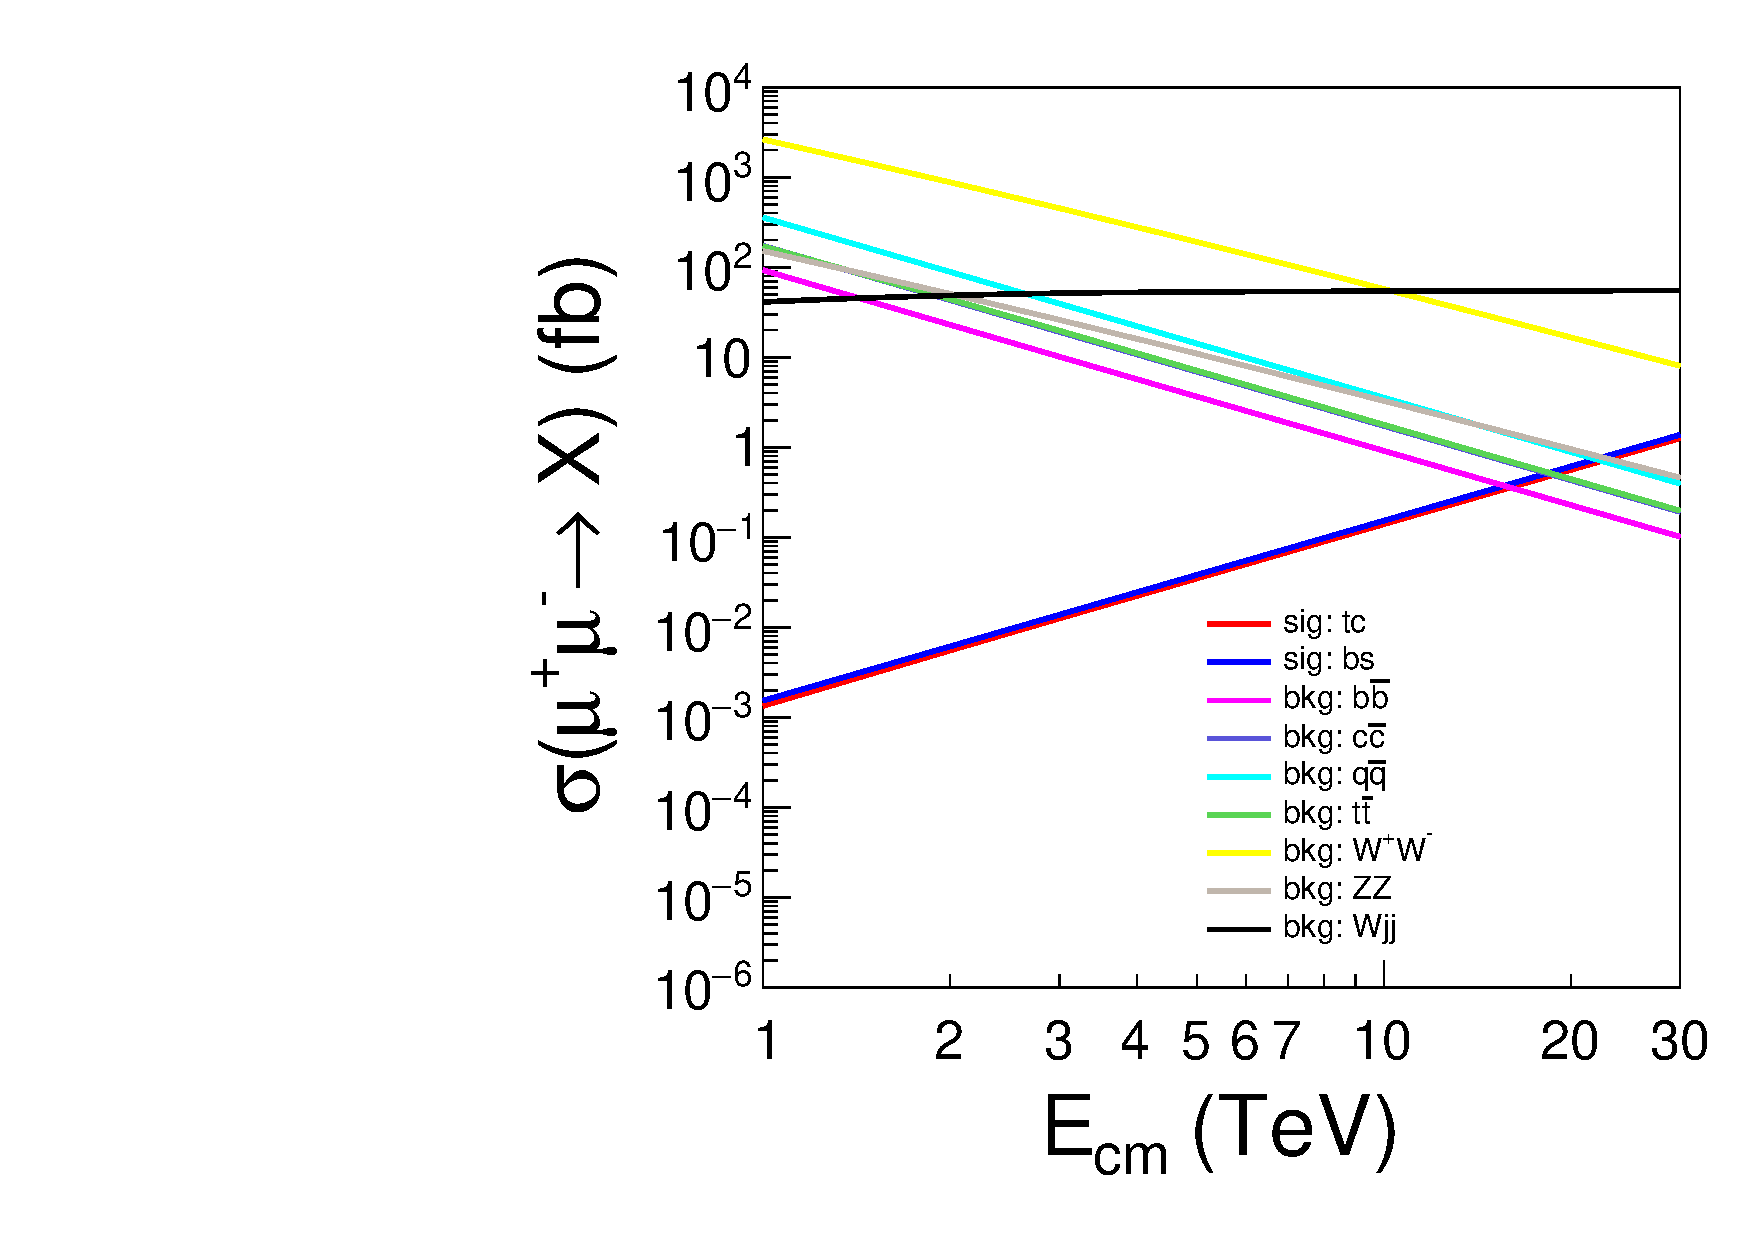
\includegraphics[width=.4\linewidth]{e_sigma_clq1_only_log.pdf}}
  \subfigure{
  \thesubfigure
  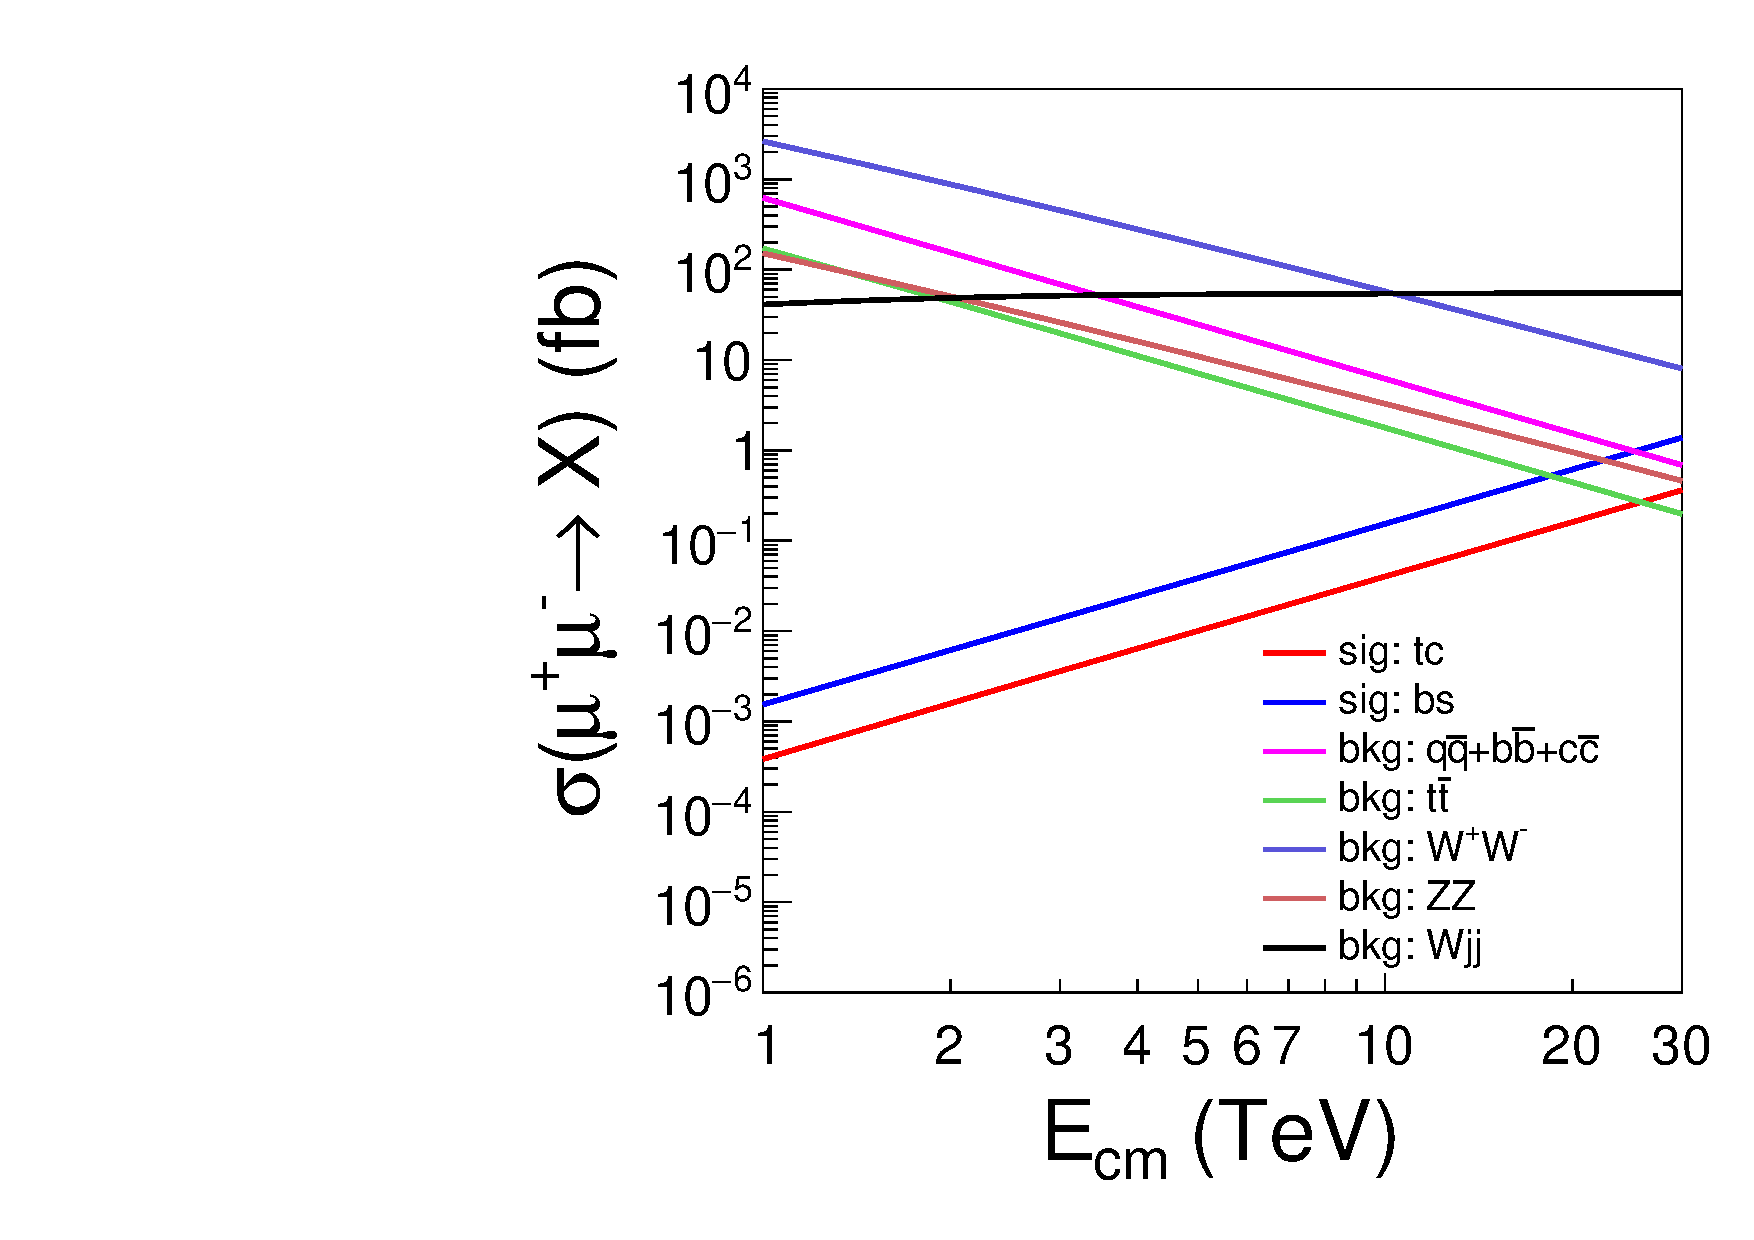
\includegraphics[width=.4\linewidth]{e_sigma_clq1_eq_3clq3_log.pdf}}
  \caption{The energy dependencies of the cross sections of $\mu^+\mu^-\to X$ are displayed. For the signal, $X=t\bar{c}$, while $X$ is the final state of the background. The best fits $c_{9}=-c_{10}=-0.39$ in Ref.~\cite{Altmannshofer:2021qrr} have been considered here. Their values are evaluated to the cutoff $\Lambda=10$ TeV by our RGEs and matching conditions in the Appendix. Two models are considered: (a) Model I, i.e. $C^{(1)}_{lq}=L^{V,LL}_{ed}\times \Lambda^2/v^2$ and $C^{(3)}_{lq}=0$,  and (b) Model II, i.e. $C^{(1)}_{lq}=3C^{(3)}_{lq}=\frac{3}{4}L^{V,LL}_{ed}\times \Lambda^2/v^2$.\label{ecm}}
\end{figure}

\begin{figure}
  \centering
  \subfigure{
  \thesubfigure
  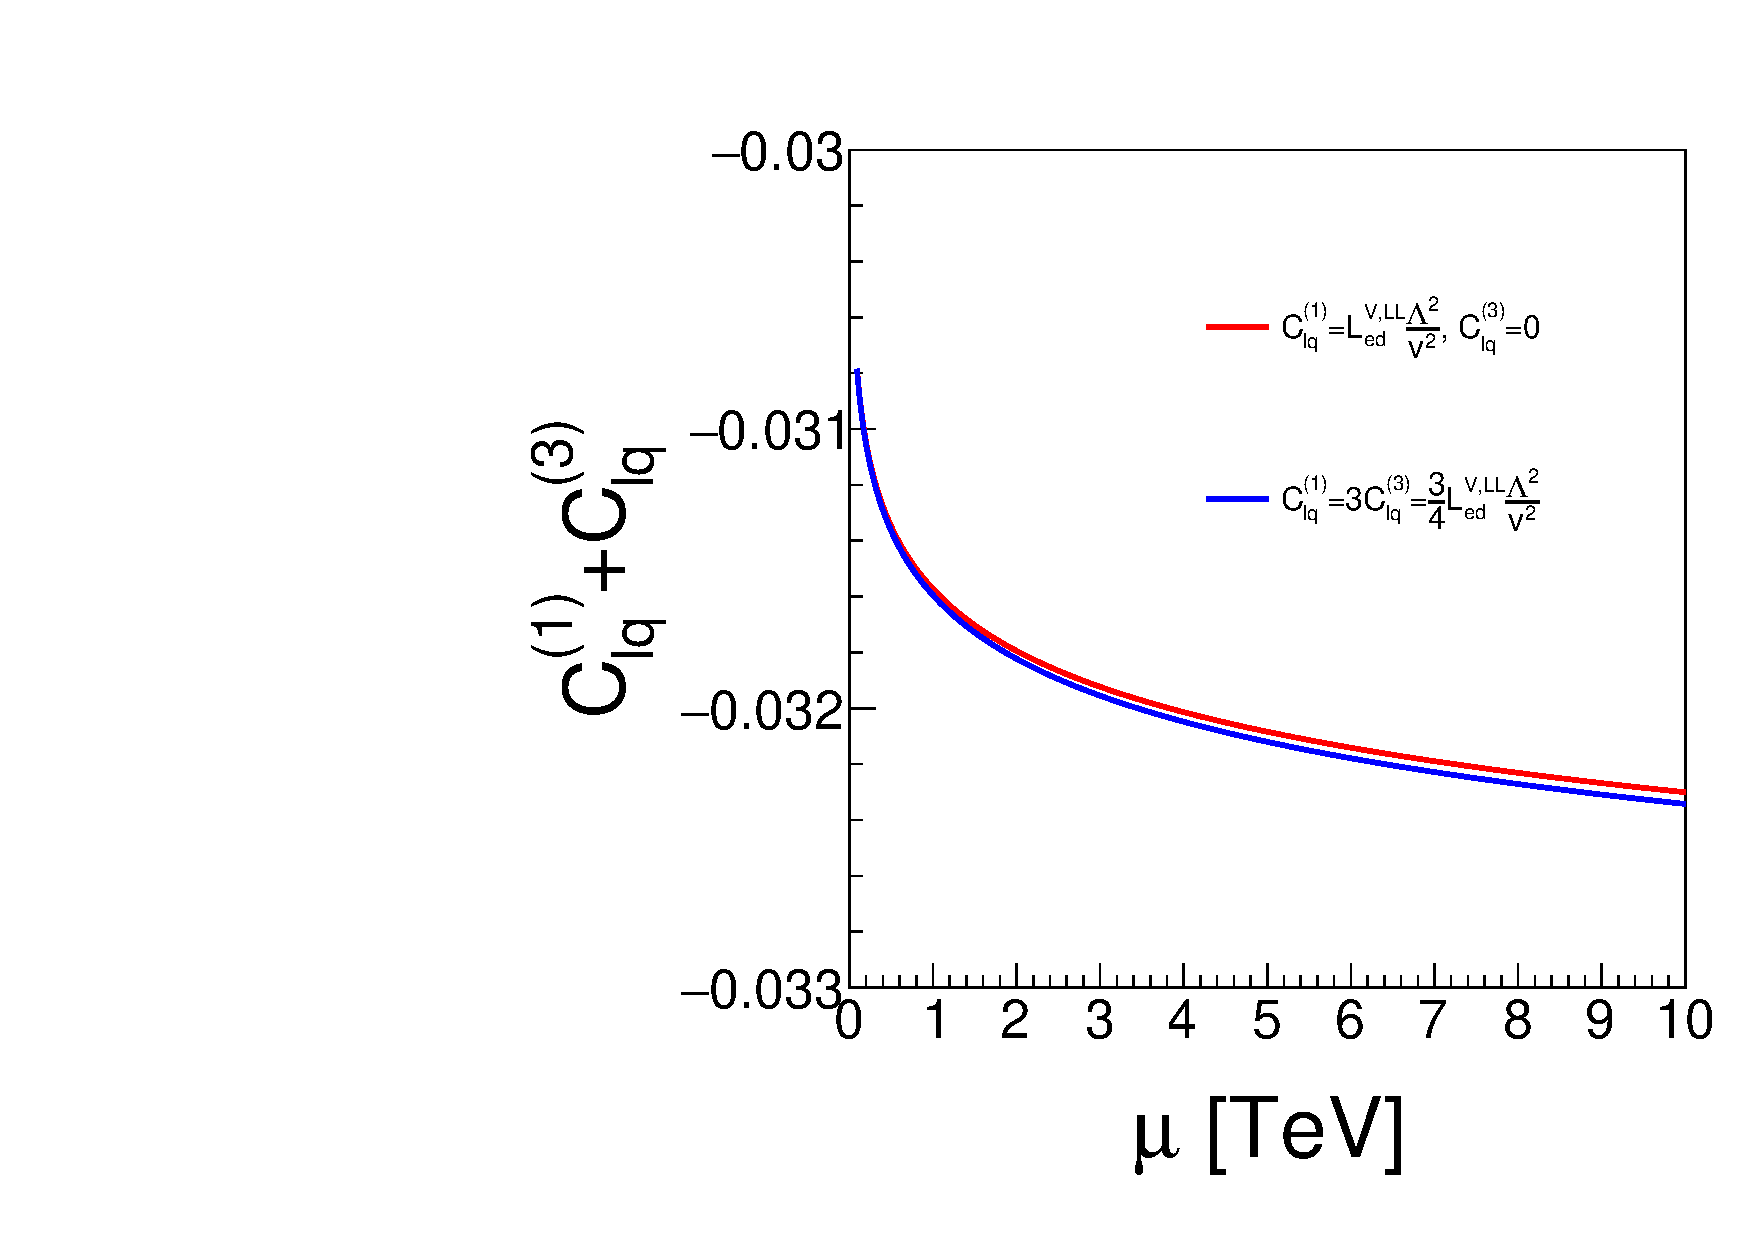
\includegraphics[width=.4\linewidth]{output_plus.pdf}}
  \subfigure{
  \thesubfigure
  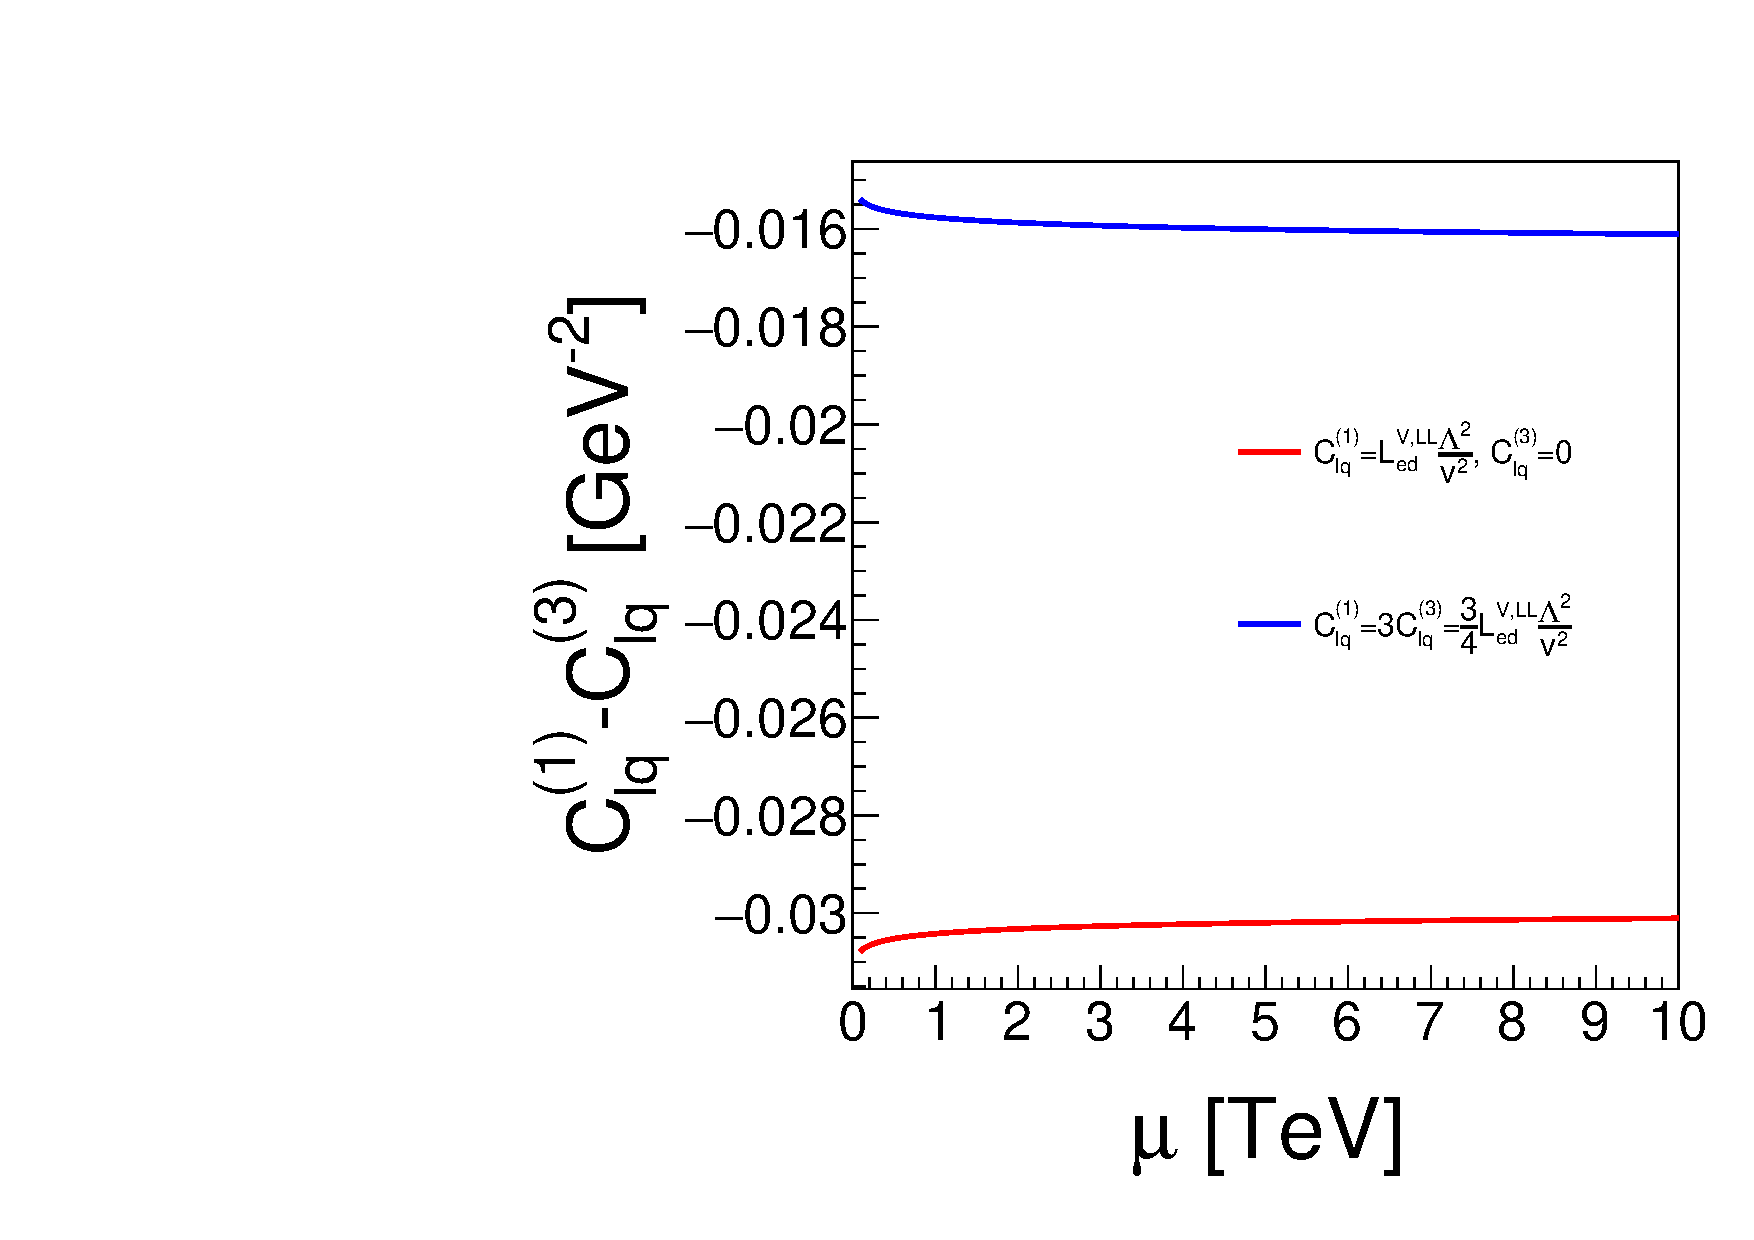
\includegraphics[width=.4\linewidth]{output_minus.pdf}}
  \caption{The running of (a) $C^{(1)}_{lq}+C^{(3)}_{lq}$ and (b) $C^{(1)}_{lq}-C^{(3)}_{lq}$ from EW scale to $\Lambda=10$ TeV is display.  Two scenarios: 1) $C^{(1)}_{lq}=L^{V,LL}_{ed}\Lambda^2/v^2$ and $C^{(3)}_{lq}=0$, and 2) $C^{(1)}_{lq}=3C^{(3)}_{lq}=\frac{3}{4}L^{V,LL}_{ed}\times \Lambda^2/v^2$ have been considered here.\label{rge:EWtoUV}}
\end{figure}

As we have seen in Fig.~\ref{ecm}, the process $\mu^+\mu^-\to t\bar{c}$ can only be observable when $E_{cm}>10$ TeV.  
In a such high energy, we can expect two energetic jets to be observed at the detector for either signal or background events. 

In Fig.~\ref{ecm}, the best fits of $c_{9}$ and $c_{10}$ in Ref.~\cite{Altmannshofer:2021qrr} have been considered. 
Their values are evaluated to the EW scale by our RGEs Eq.~\ref{beta:VLLed} and Eq.~\ref{beta:VLRde}. 
And then they are matched to SMEFT by Eq.~\ref{match:VLLed} and Eq.~\ref{match:VLRde}. 
From Eq.~\ref{match:VLLed}, we also know that the constraint from B physics can be only applied to the sum of $C^{(1)}_{lq}+C^{(3)}_{lq}$~\footnote{The generation indices are always $(p,r,s,t)=(2,2,2,3)$ for $C^{(1)}_{lq}$ and $C^{(3)}_{lq}$ and $(p,r,s,t)=(2,3,2,2)$ for $C_{qe}$ in this paper.}.  
So any new physics scenarios with $C^{(1)}_{lq}$ and $C^{(3)}_{lq}$ as free parameters cannot be constrained by the data from B physics experiments. 
In Fig.~\ref{rge:EWtoUV}, we show the running of $C^{(1)}_{lq}+C^{(3)}_{lq}$ and $C_{qe}$ from EW scale to new physics scale at $\Lambda=10$ TeV, 
in the case of $c_{9}=-0.73$ and $c_{10}=0$.
We have considered two simple scenarios: 1) $C^{(1)}_{lq}=L^{V,LL}_{ed} \frac{\Lambda^2}{v^2}$ and $C^{(3)}_{lq} = 0$; 2) $C^{(1)}_{lq}=3 C^{(3)}_{lq}=\frac{3}{4} L^{V,LL}_{ed} \frac{\Lambda^2}{v^2}$\xznote{At which scale?}.
Considering the experimental uncertainties, it is challenging to distinguish these two cases from RGE running. 

\subsection{Jet Level Analysis}

It should be mentioned that for a muon collider, 
the collision environment is relatively clean and there is no serious pileup and underlying event which occurred at a hadron collider, 
but there exist beam-induced backgrounds which arise from the muon decay. 
By using the jet grooming techniques, 
it is possible to suppress such beam-induced backgrounds \cite{Collamati:2021sbv}. 
Therefore, we will neglect the beam induced backgrounds in our study.

Meanwhile, since it is more and more realistic to use the particle flow method to measure the jet energy, 
which can reduce the uncertainty of jet energy down to $5\%-20\%$ \cite{Nachman:2022emq}. 
Actually, one benefit of the particle flow method can also help us to distinguish a light jet, 
a W/Z boson jet, and a top jet: a W/Z/top jet can have more charged tracks in a detector when compared with a light jet.

To further investigate the kinematic features of jets from signal processes, 
we use PYTHIA8~\cite{Bierlich:2022pfr} for parton shower and hadronization, 
and FastJet~\cite{Cacciari:2011ma} to reconstruct jets.  
It is expected that jet algorithms developed for electron-positron colliders can also be applied well to muon colliders. 
Therefore, we use the generalised $k_t$ algorithm for $e^+e^-$ collisions,
which is extended from a simple $k_t$ algorithm~\cite{Catani:1991hj}.
This algorithm defines two distances:
\begin{eqnarray}
  d_{ij} &=& \min(E^{2p}_i,E^{2p}_j)\frac{1-\cos\theta_{ij}}{1-\cos{R}}, \label{eq:genkt1}\\
  d_{iB} &=& E^{2p}_i, \label{eq:genkt2}
\end{eqnarray}
where $p$ and $R$ are input by user. If a $d_{ij}$ is smallest then particle $i$ and $j$ are recombined, while $d_{iB}$ is smallest then $i$ is called an "inclusive jet''.
In this context, we choose $p=1$.

It should be pointed out that the denominator $(1-\cos{R})$ is replaced by $(3+\cos{R})$ while choosing $\pi<R<3\pi$ in FastJet.
In this case, $d_{iB}$ is always larger than $d_{ij}$ so that only one inlcusive jet can be found.  
If we also choose $p=1$, the generalised $k_t$ algorithm is identital to the original $k_t$ algorithm~\cite{Catani:1991hj}, 
which only has a single distance:
\begin{eqnarray}
  d_{ij} &=& \min(E^{2}_i,E^{2}_j)\left(1-\cos\theta_{ij}\right), \label{eq:eekt}
\end{eqnarray}
and one can extract ``exclusive jet'' only. 
For the high energy muon collider, muon beams may radiate energetic particles which can have large angles to the beams. 
Such kind of particles are included in the exclusive jets. 
So this algorithm is not sufficient in our context.

Below we will demonstrate a case study with the collision energy $\sqrt{s}=10$ TeV at the jet level analysis. We demand all signal and background events have hadronic decays and neglect those semi-leptonic and pure leptonic final states. 

Since the dominant background processes are $WW (ZZ)$, $tt$, 
and $jj$ which can have more than two energetic jets in the final state, 
in order to avoid the combinatoric issues, it is better to have less number of jets in the final state. 
For example, when $R=0.05$ and $E_j>100$\xznote{Inconsistency!Later $E_j>500$ is adopted}, 
the number of jets for a signal event can be much more than $10$, which is difficult to analyze. 
Then appropriate jet parameters, like cone parameter and energy cut, 
are crucial for the jet numbers and the preselection of signal events. 
Due to the fact that both $W/Z$ bosons and top quarks are highly boosted in the final state 
(each of them carries an energy 5 TeV), 
it is crucial to set the value of jet parameter so as to capture the whole decay products of $W/Z$ bosons and top quarks. 
Therefore, in this study, we will focus on the boosted events in our analysis.

According to the rule of thumb, the typical cone parameter for a top jet with a large $P_t$ can be expressed as $R_t = \frac{2 m_t}{P_t}$. 
\xznote{Wrong formula! This is for the algorithm which uses $P_t$, while here we are using $E$!} 
It can be estimated that all products of a $P_t=3.5$ TeV top jet can collimate in a cone with value $R_t= 0.1$ or so. 
Considering that the future ECAL (HCAL) detector can have a granularity with $\Delta \eta \times \Delta \phi = 0.01 \times 0.009 (0.025 \times 0.025)$ for the FCC-hh detector \cite{FCC:2018vvp}, 
\xznote{Wrong detector!} there is no doubt that a future detector of a muon collider is able to resolve the substructure of such a highly boosted top jet. 

The optimization of parameters $p$ and $R$ is a complicated task.
As a first attempt, we choose $p=1$ so it works similarly to a $k_t$ algorithm for hadron collider~\cite{Catani:1993hr,Ellis:1993tq}. 
For the $t\bar{c}(\bar{t}c)$ final state, we hope to find a $R$ parameter to reconstruct a heavy jet around top mass and a light jet.
We have scanned the $R$ parameter from $0.05$ to $0.15$ and have found that $R=0.10$ can satisfy this requirement. 

In Fig.~\ref{subfig:ej_tc}, we display the energy distribution of the leading three jets in $t\bar{c}(\bar{t}c)$ final with $R=0.10$ and $p=1$. 
These jets are sorted by energy.  Obviously, the first two jets have energy around $E_{cm}/2$, 
which means that they probably originated from a hard process.
We can also observe that the energy of the 3rd jet can reach several hundred GeV or TeV levels.
In such a high energy collider, parton shower can radiate some high energy particles and can be detected as a hard jet. To reduce these radiations, we implement a cut $E(j)>500$ GeV to jets for each event. 
After this cut, we plot the number of jets in Fig.~\ref{subfig:njets}. 
As we can see, the peak is $N_{jets}=2$ for two final state processes, and the peak for $W^{\pm}jj$ background is 3.  Therefore to demand the number of jets $N_j=2$ for each event can heavily suppress the background events of $\mu^+ \mu^0 \to W^{\pm}jj$.

\begin{figure}[htbp]
%  \setcounter{subfigure}{0}
  \centering
  % Requires \usepackage{graphicx}
  \subfigure{
  \thesubfigure
  \label{subfig:ej_tc}
  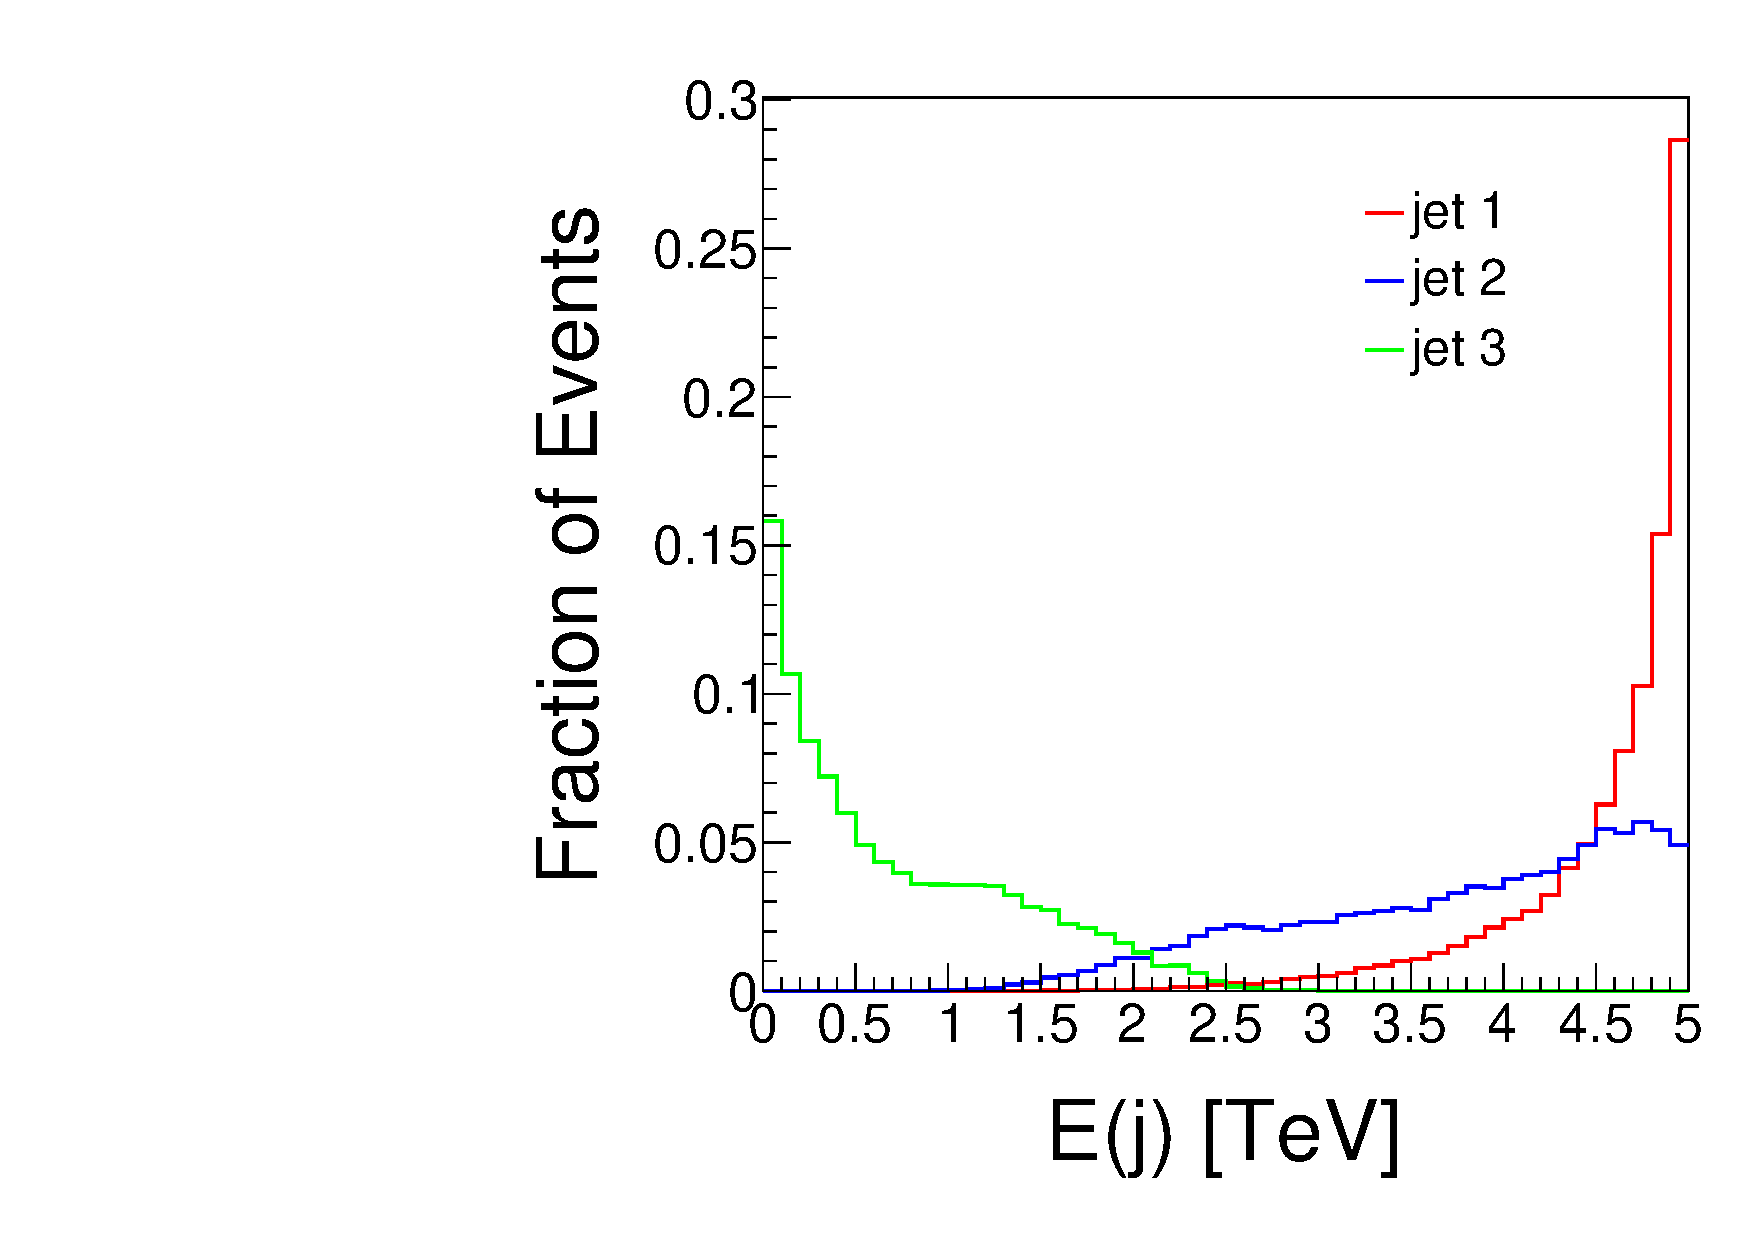
\includegraphics[width=0.4\textwidth]{ej_tc.pdf}}
  \subfigure{
  \thesubfigure
  \label{subfig:njets}
  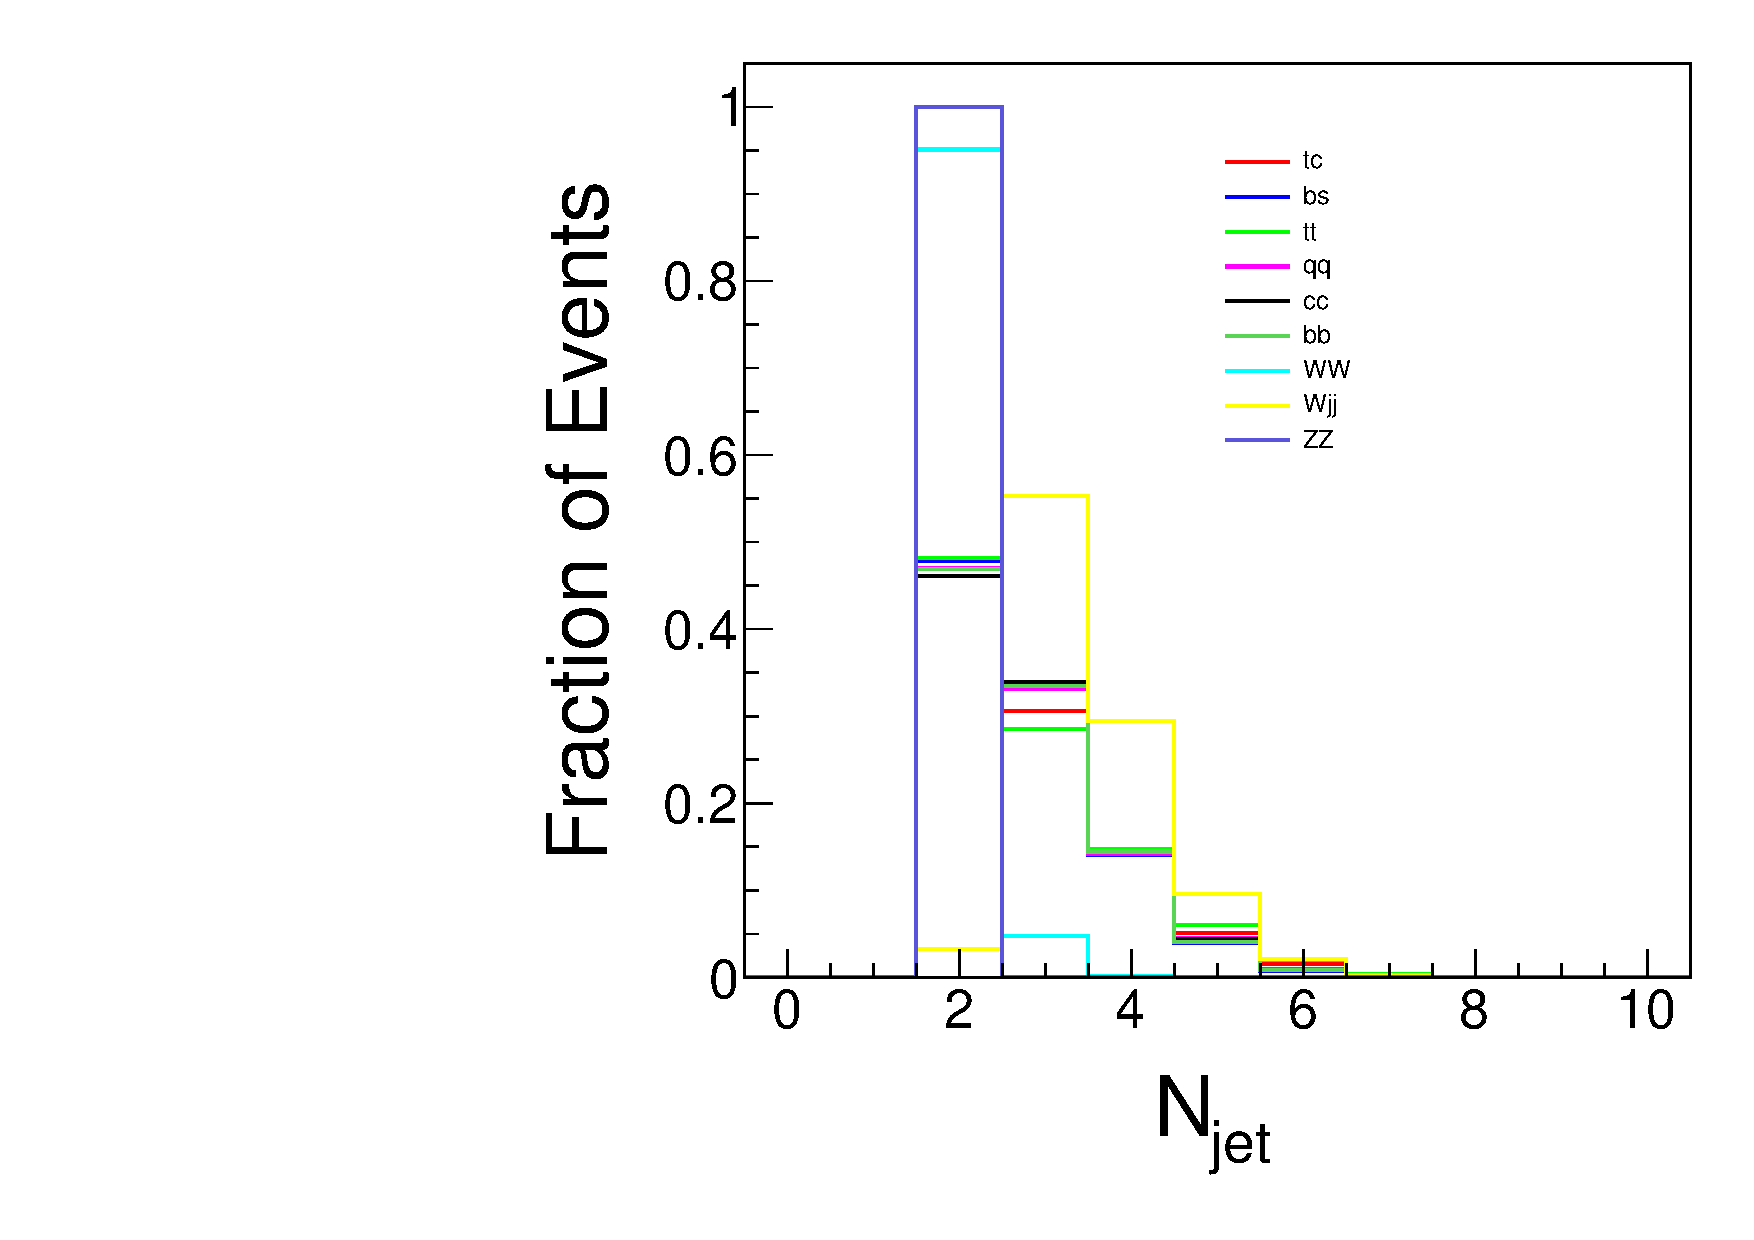
\includegraphics[width=0.4\textwidth]{njets.pdf}}
  \caption{(a) The jet energy distributions of process $\mu^+\mu^-\to t\bar{c}$ are displayed, where jets are sorted by energy. (b) The number of jets after implementing cut $E(j)>500$ GeV.}\label{fig:base}
\end{figure}

Fig.~\ref{fig:mj1mj2} shows the invariant masses of the two most energetic jets of signal and background events. 
Here, we label the heavier jet as HJ in Fig.~\ref{fig:mj1} and the lighter one as LJ in Fig.~\ref{fig:mj2}.
As we expect, HJ has a peak around the top mass and the distribution of LJ is flat for the signal.
For the backgrounds with heavy particles ($t$, $W$, and $Z$), we also observe peaks around their masses. 
It is because these particles are highly boosted in such a high energy machine. 
%We can include all their decayed products by choosing a small jet cone like $R=0.10$.

\begin{figure}[htbp]
  \setcounter{subfigure}{0}
  \centering
  % Requires \usepackage{graphicx}
  \subfigure{
  \thesubfigure
  \label{fig:mj1}
  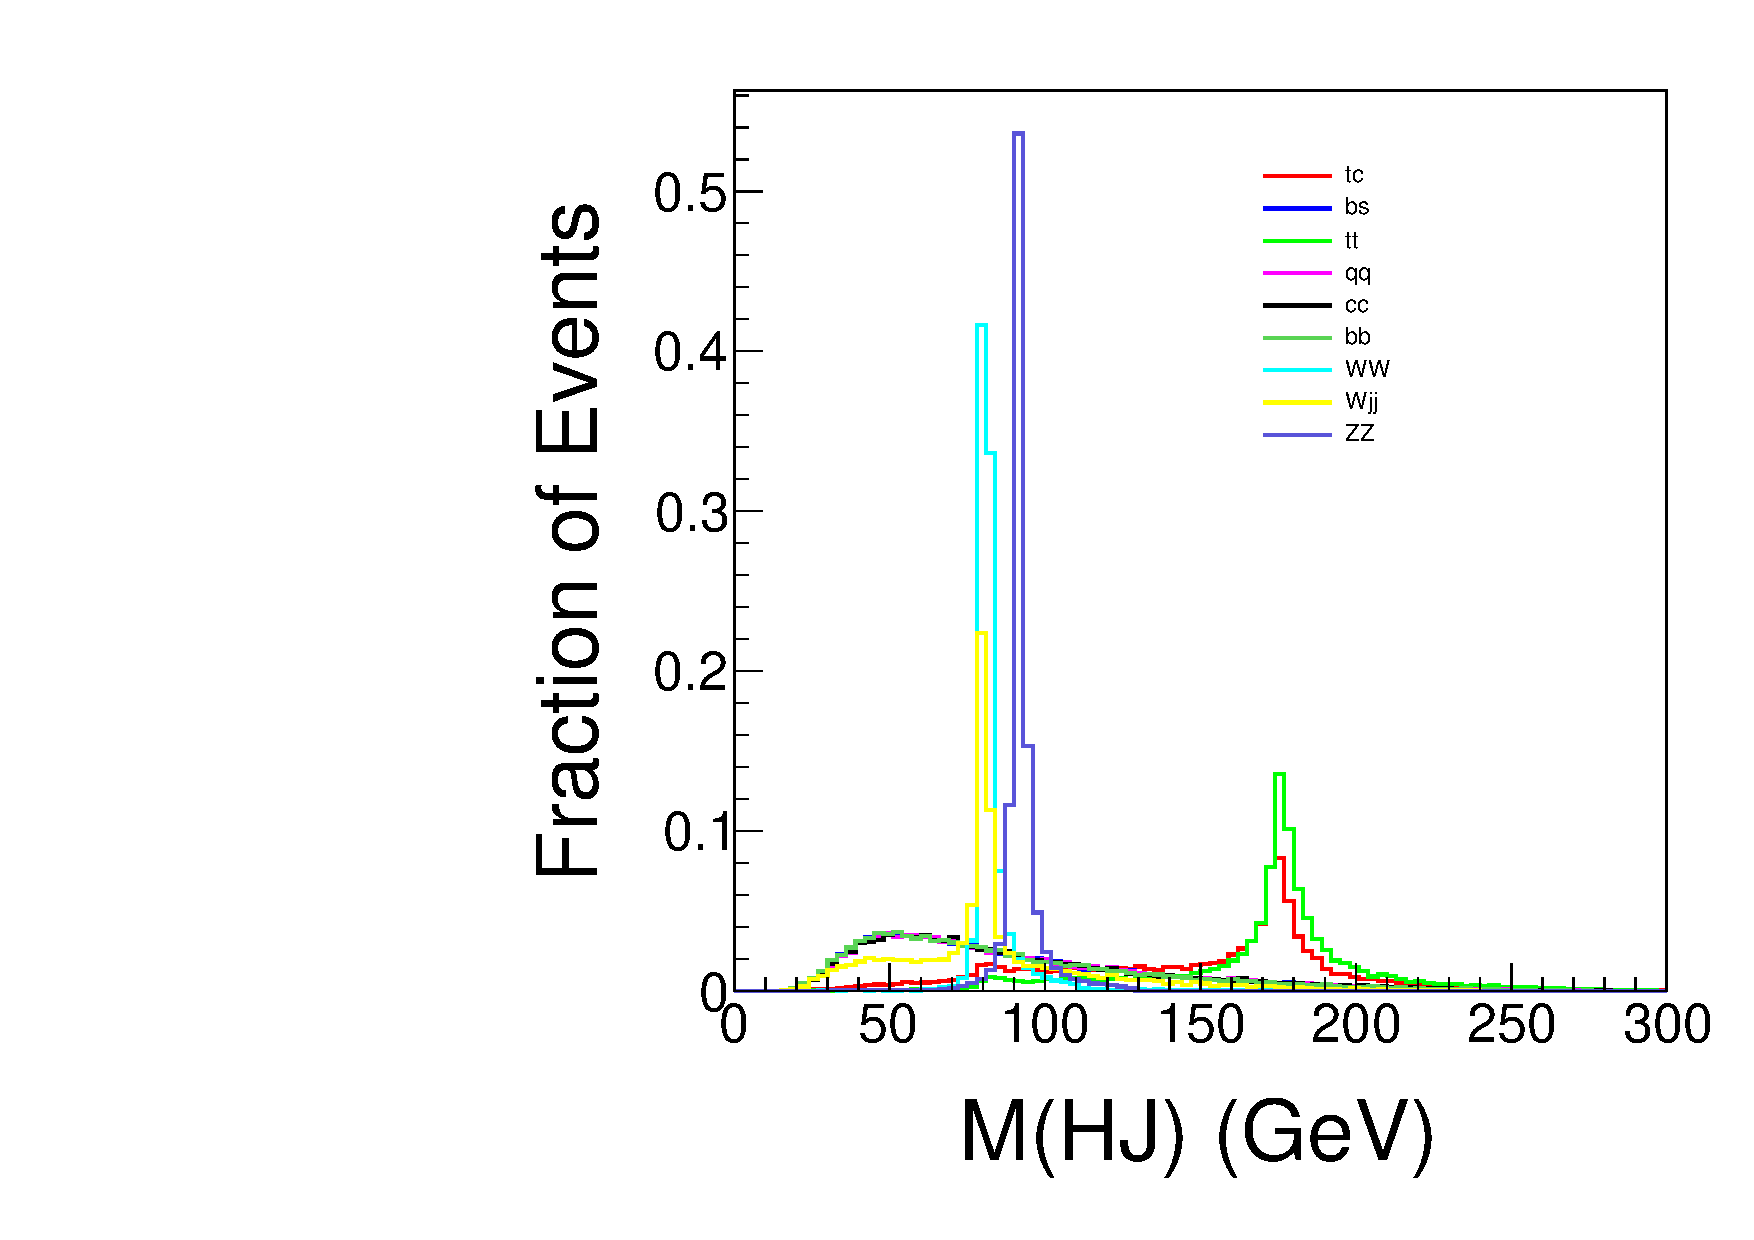
\includegraphics[width=0.4\textwidth]{mj1.pdf}}
  \subfigure{
  \thesubfigure
  \label{fig:mj2}
  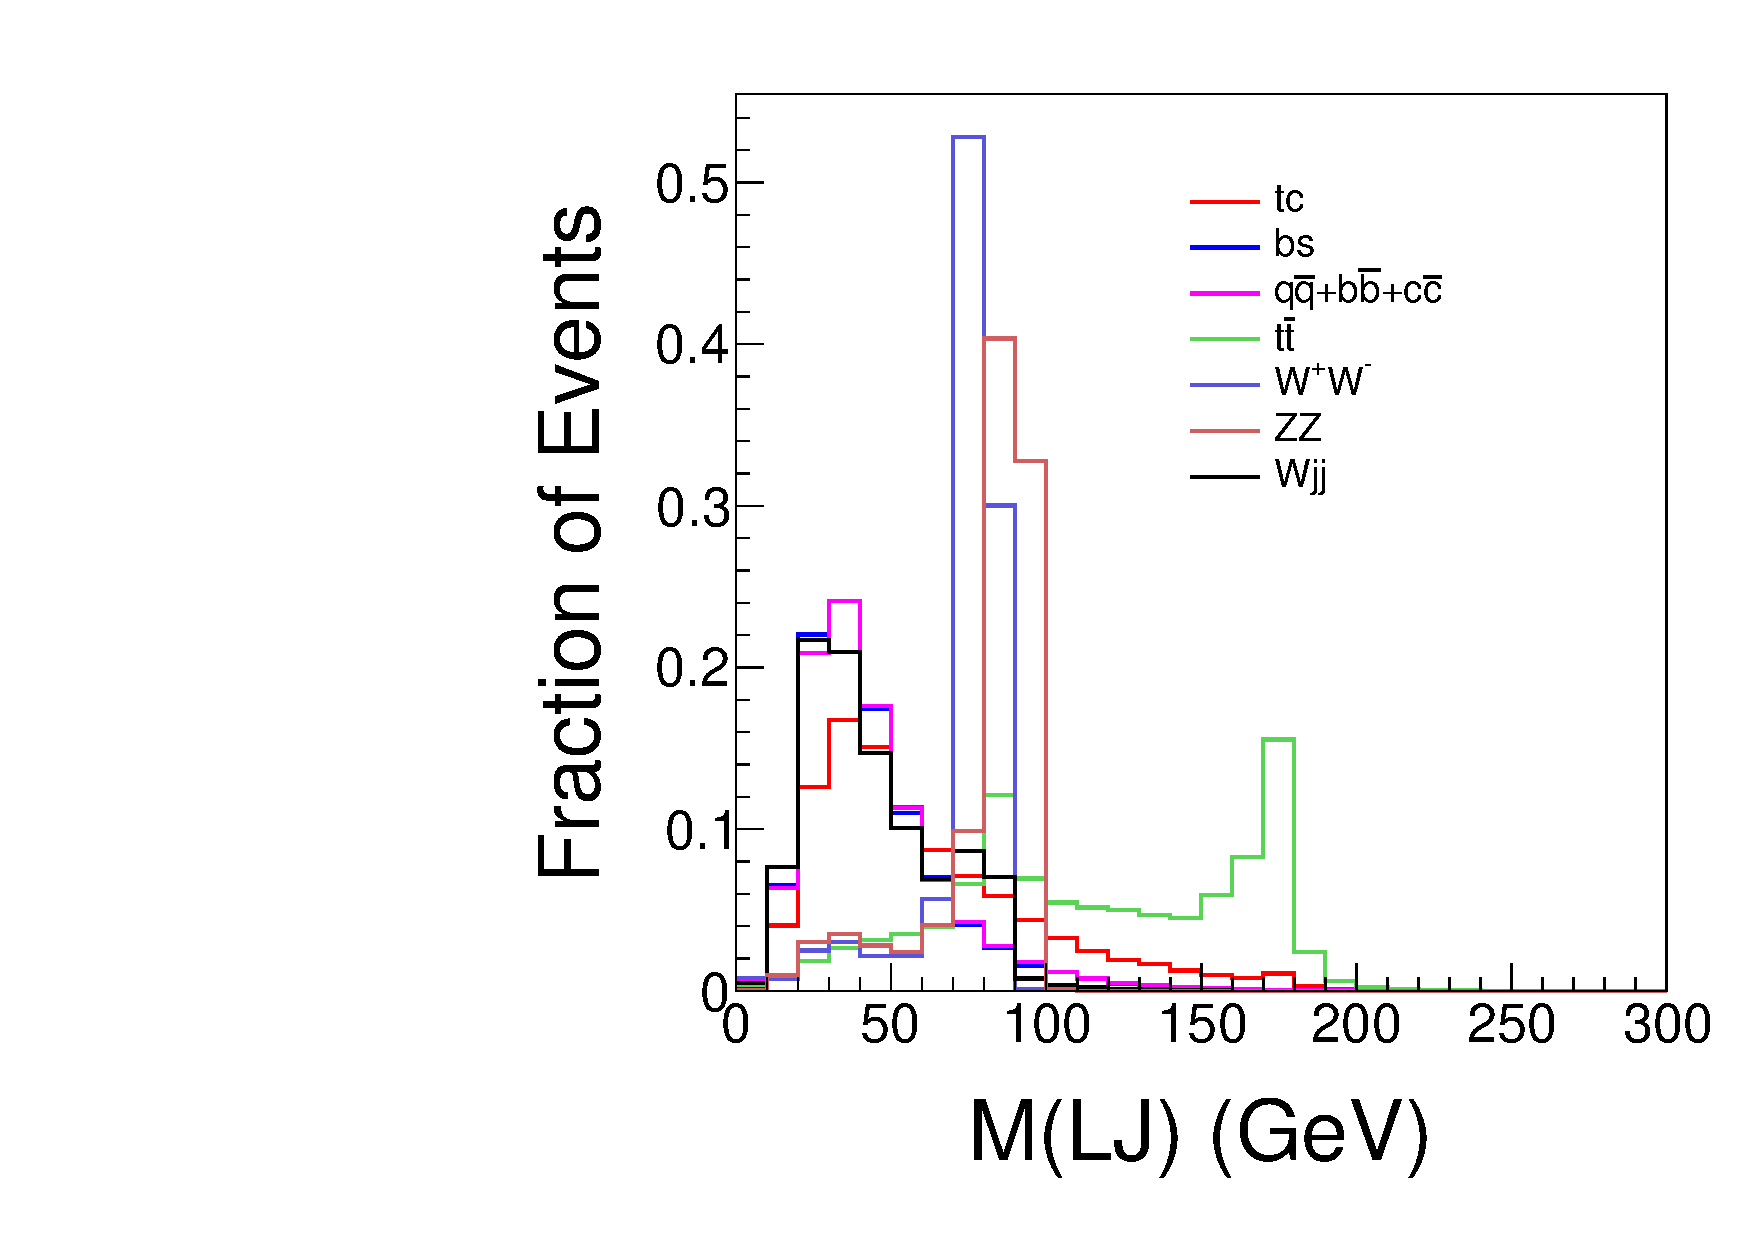
\includegraphics[width=0.4\textwidth]{mj2.pdf}}
  \caption{The invariant mass of (a) the heavier jet and (b) the lighter jet in signal and backgrounds are displayed.}\label{fig:mj1mj2}
\end{figure}

B-tagging and C-tagging techniques can help signal and background separation. 
As shown in \cite{ATLAS:2019bwq}, the larger the transverse momentum, the better the B tagging efficiency. 
Therefore we expect a higher B-tagging efficiency for a 10 TeV collision. 
Although B mesons and D mesons have similar proper times at $10^{-12}$ seconds, their masses are different. 
If C-tagging techniques \cite{ATLAS:2021cxe} can be applied in our analysis, we expect better results can be obtained. 

Since we only consider hadronic decay, the top quark should decay to $b$ quark and $W$ boson, 
and $W$ further decays to light quarks. 
So the HJ of a signal event should also be tagged as a $b$-jet in a future detector. 
%In this paper, the detector simulation is not performed. 
To consider the $b$-tagging effects, we track all decayed products of $b$-hadrons after the hadronization. 
If the constituents of a jet have a b-hadron, we can label this jet is a true $b$-jet. 
The same procedure can be applied to label $c$-jet. 

Fig.~\ref{fig:nbjets} and Fig.~\ref{fig:ncjets} show the number of true $b$-jets and $c$-jets for signals and backgrounds with quarks.
Obviously, a $b$-jet and a $c$-jet are found in the $t\bar{c}(\bar{t}c)$ signal. 
For backgrounds with two b quarks ($t\bar{t}$ and $b\bar{b}$), two $b$-jets can be found in most events.
For the $c\bar{c}$ backgrounds, most events include two $c$-jets.
Most of the $q\bar{q}$ events do have not both $b$- and $c$-jet, 
but a small fraction of such events can have $b$- or $c$-jets in the final state.  
For example, in the parton shower, a quark has a certain probability to radiate a gluon, 
and subsequently, this gluon may split to heavy quarks like $b\bar{b}$ and $c\bar{c}$. 
Such a kind of process is easier to occur for an energetic light quark,  
which may lead to an increase in the mistagging rate of light quarks. 
For backgrounds with gauge bosons, as we plot in Fig.~\ref{fig:nbjets_wz} and Fig.~\ref{fig:ncjets_wz}, 
$ZZ$, $W^+W^-$ or $W^{\pm}jj$ can decay to $b$ or $c$ quark, 
so we also observe some $b$- or $c$-jets are found in these events.

With this flavor tagging information, we can implement a $b$-tagging cut. In our analysis, the $b$-tagging rate is $\epsilon_{b}=0.7$, while the mistagging rate is $\epsilon_{c}=0.1$ and $\epsilon_{q}=0.01$ for $c$-jets and light jets, respectively.

\begin{figure}[htbp]
  \setcounter{subfigure}{0}
  \centering
  % Requires \usepackage{graphicx}
  \subfigure{
  \thesubfigure
  \label{fig:nbjets}
  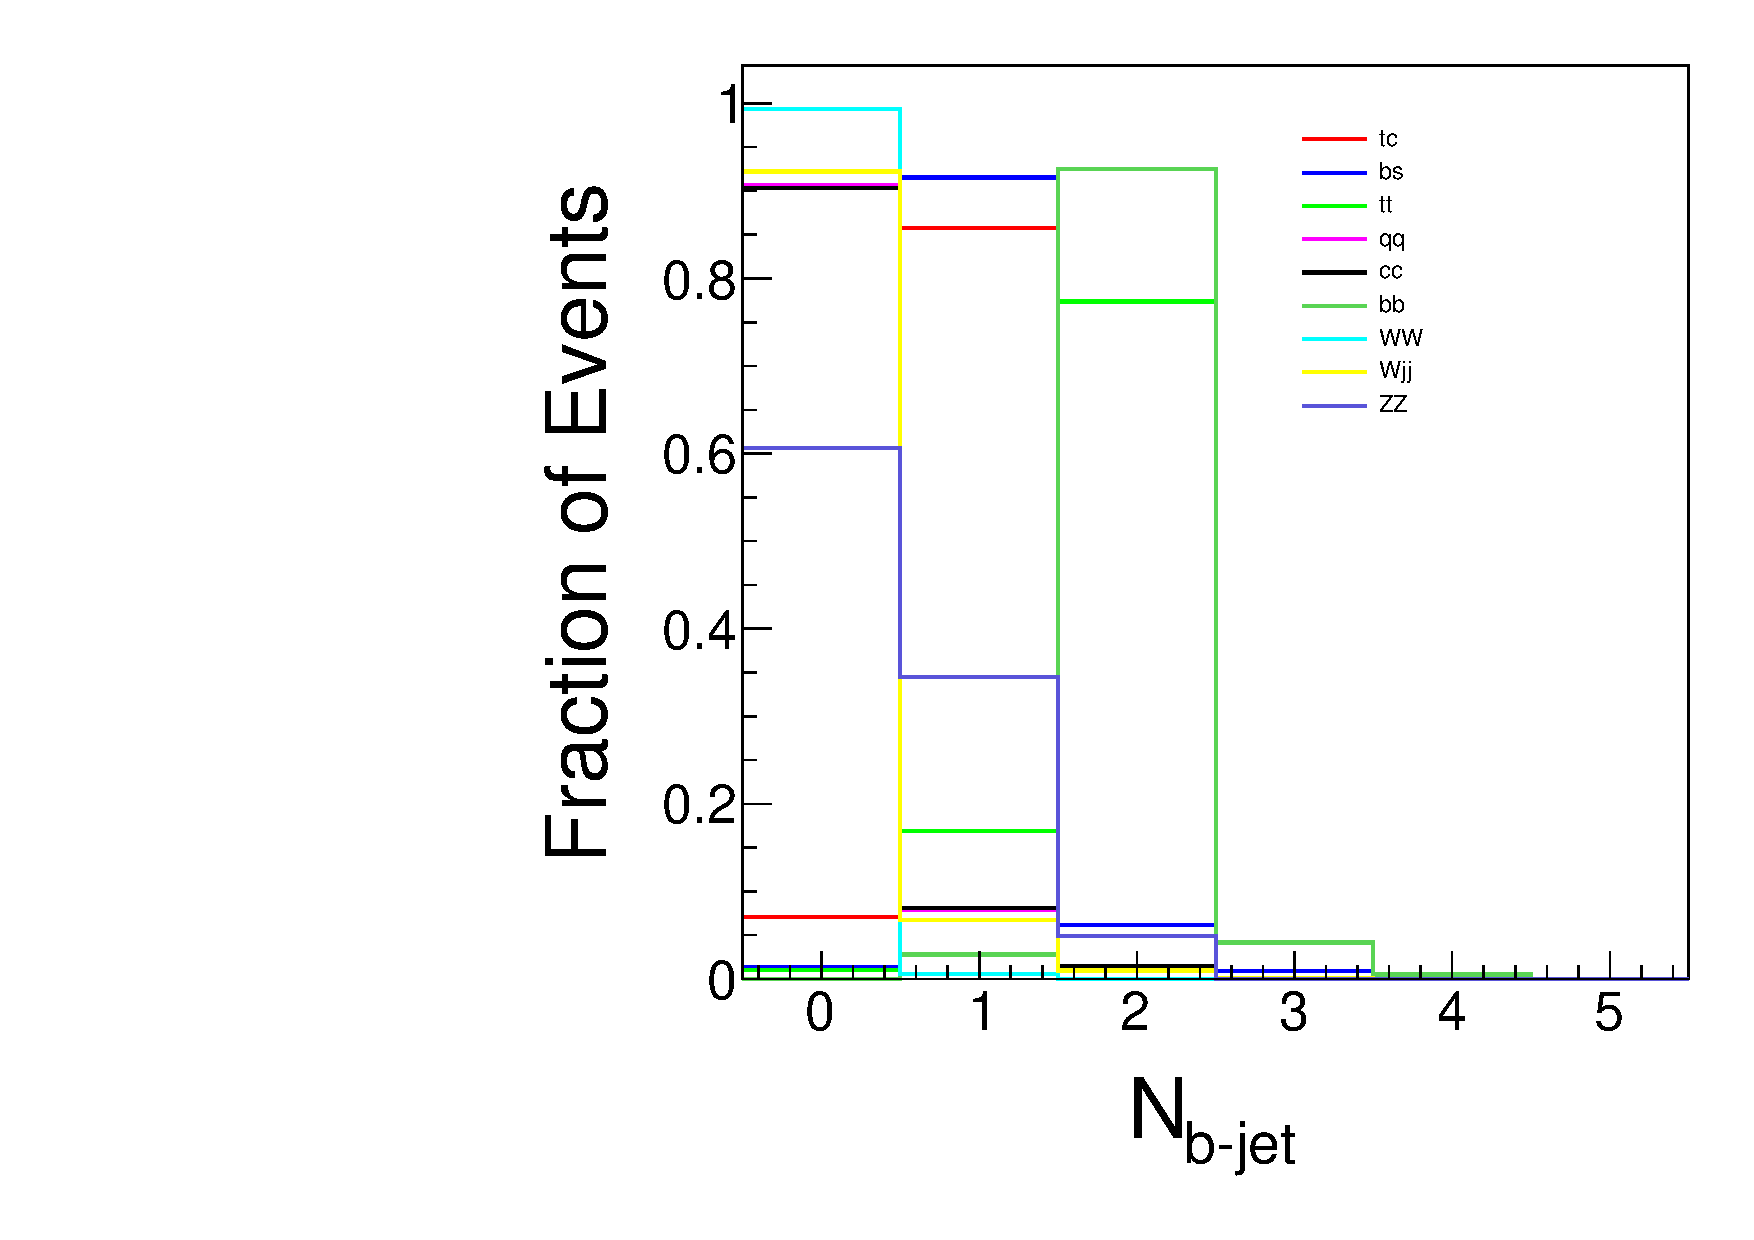
\includegraphics[width=0.4\textwidth]{nbjets.pdf}}
  \subfigure{
  \thesubfigure
  \label{fig:ncjets}
  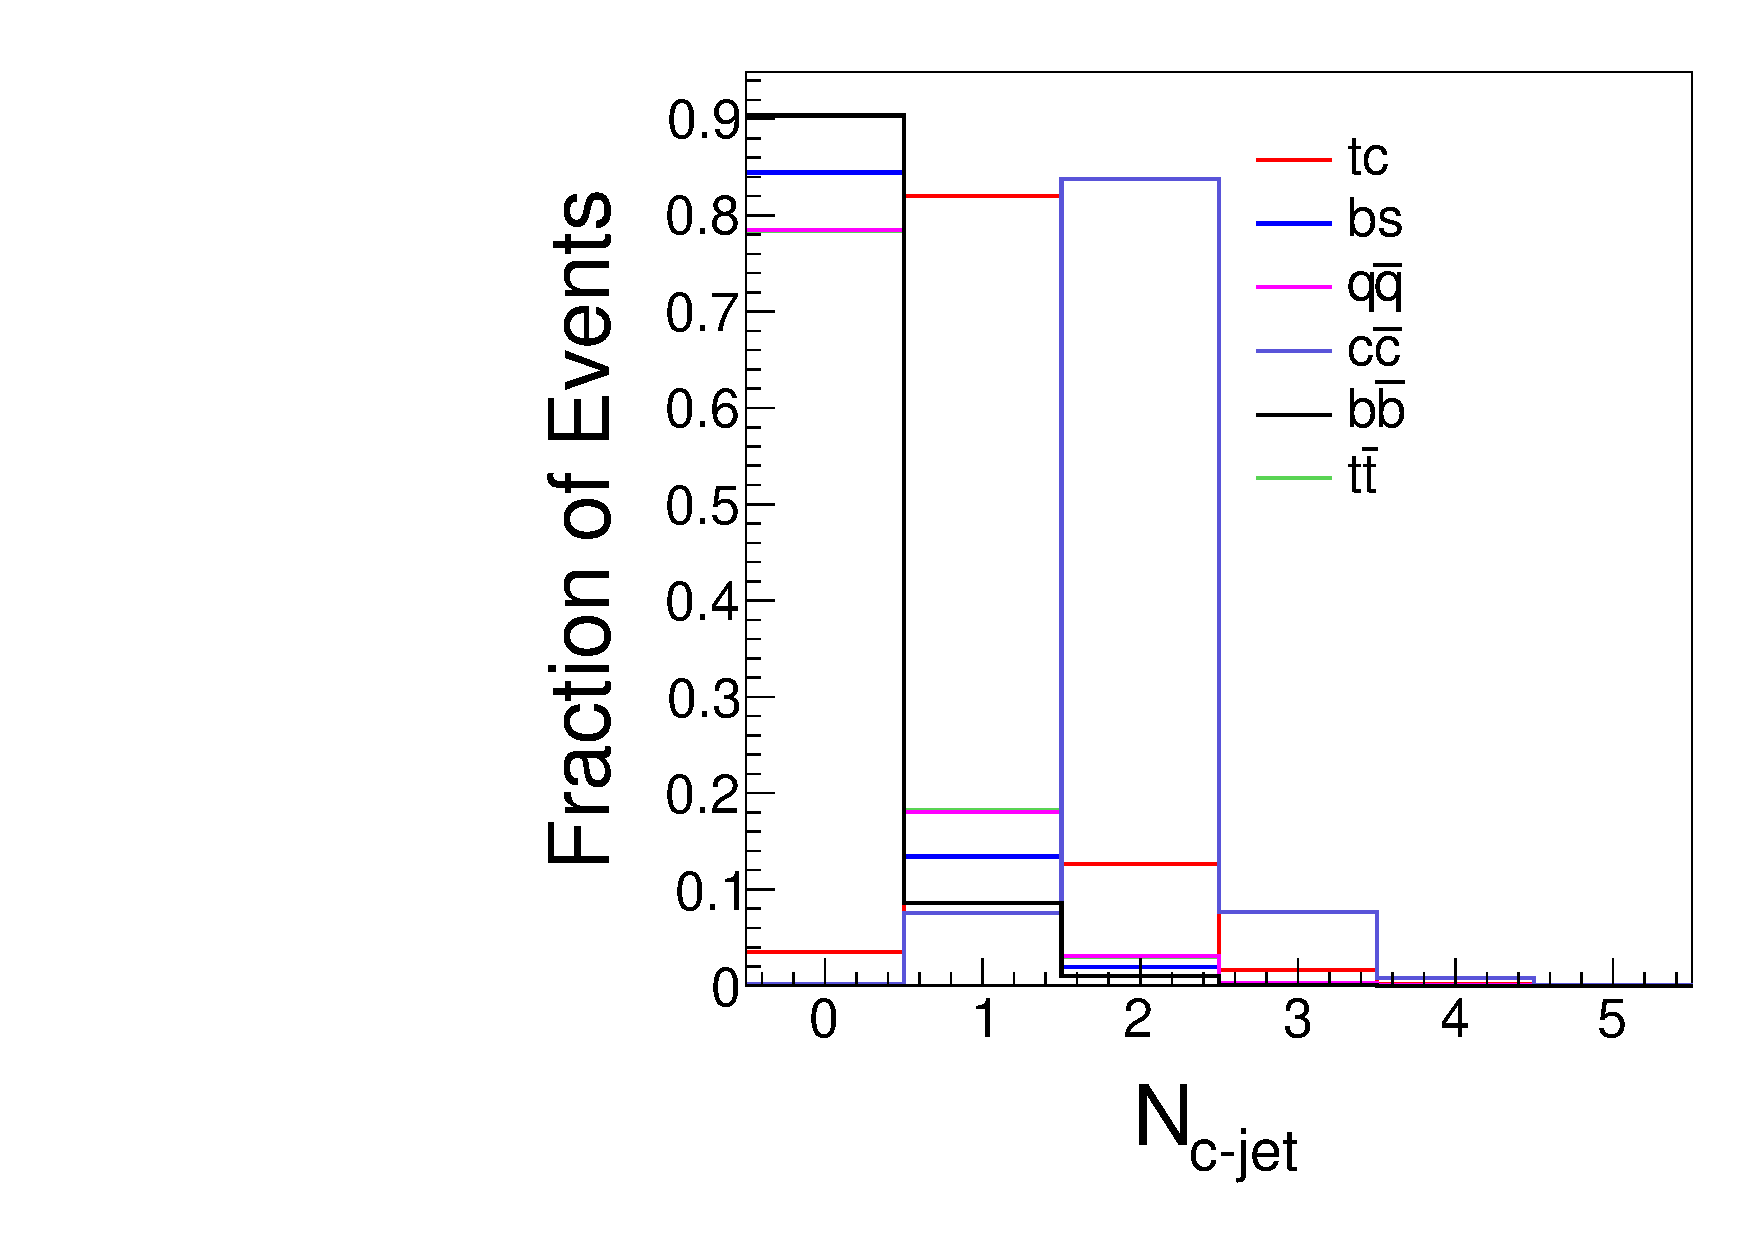
\includegraphics[width=0.4\textwidth]{ncjets.pdf}}
  \subfigure{
  \thesubfigure
  \label{fig:nbjets_wz}
  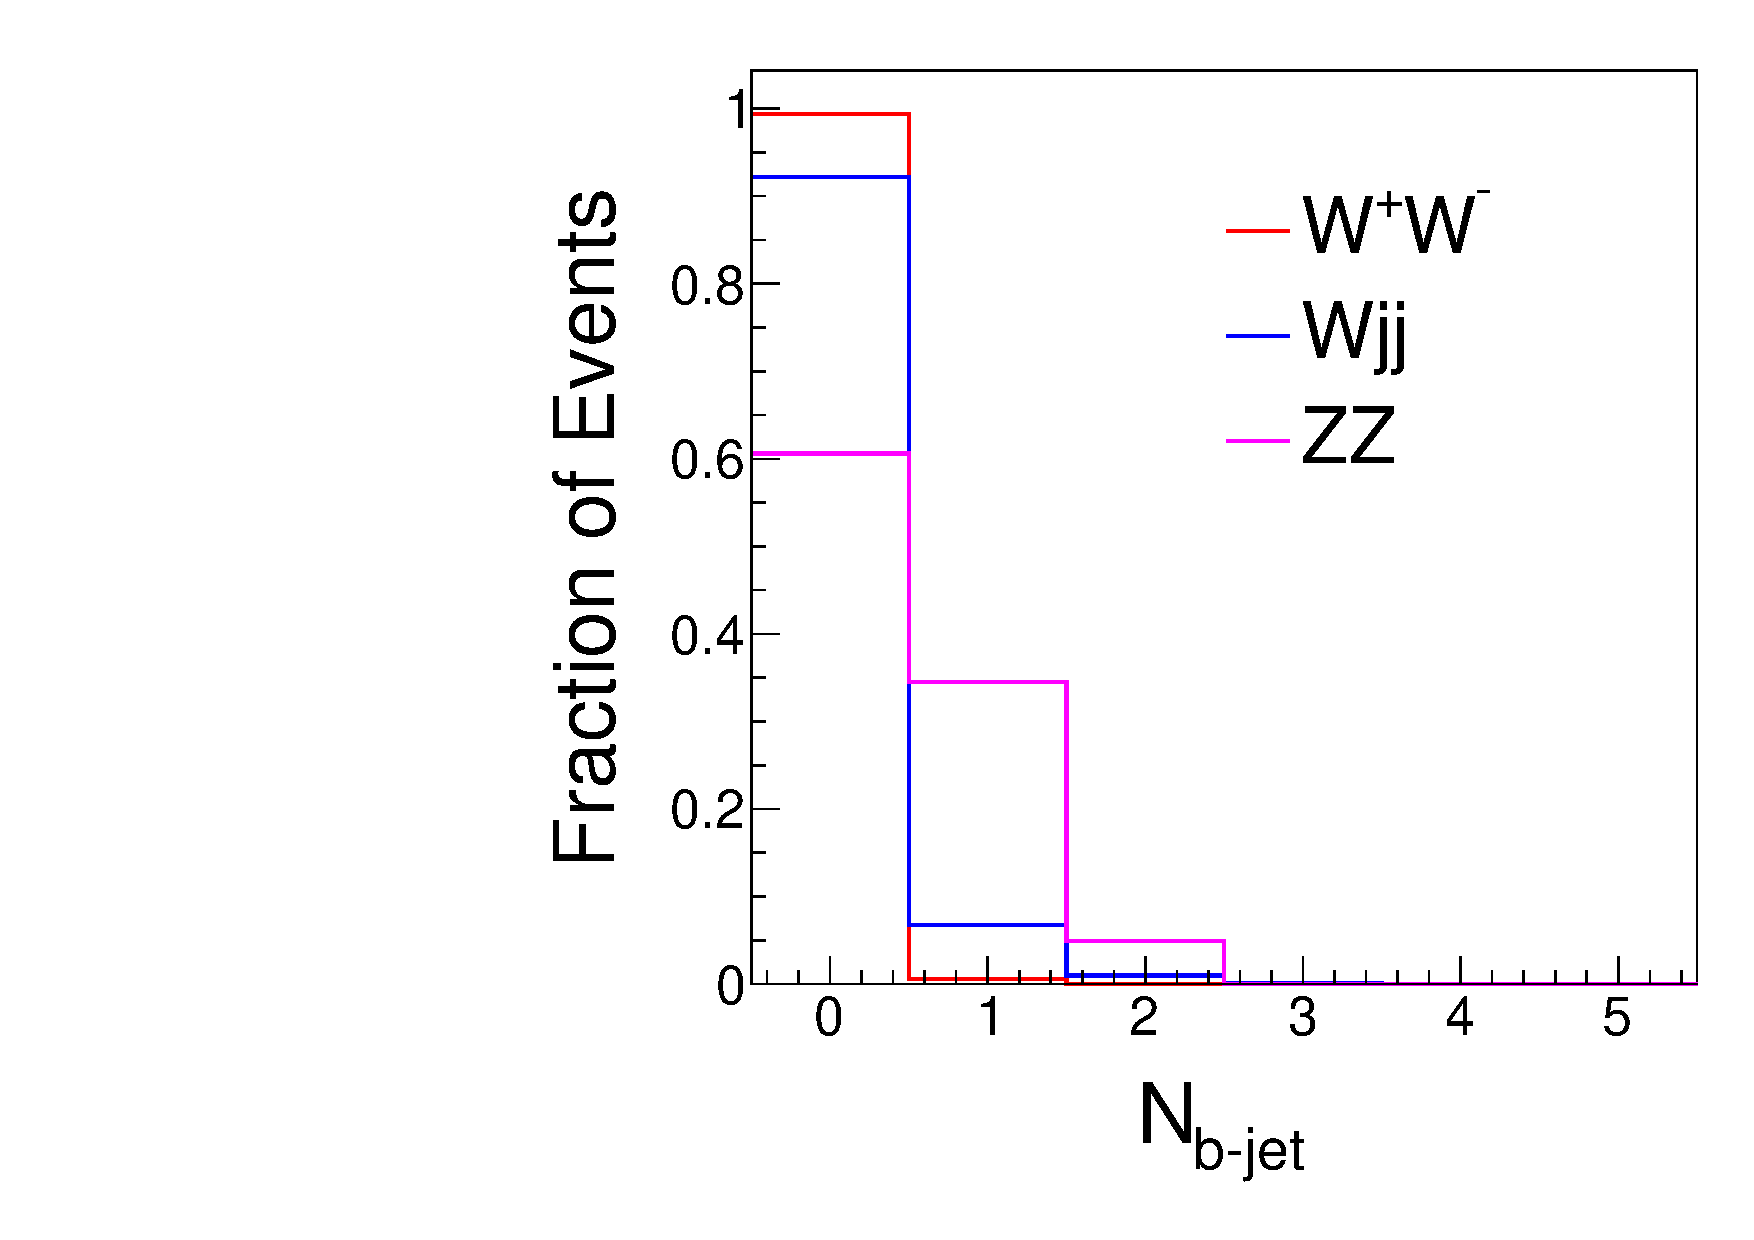
\includegraphics[width=0.4\textwidth]{nbjets_wz.pdf}}
  \subfigure{
  \thesubfigure
  \label{fig:ncjets_wz}
  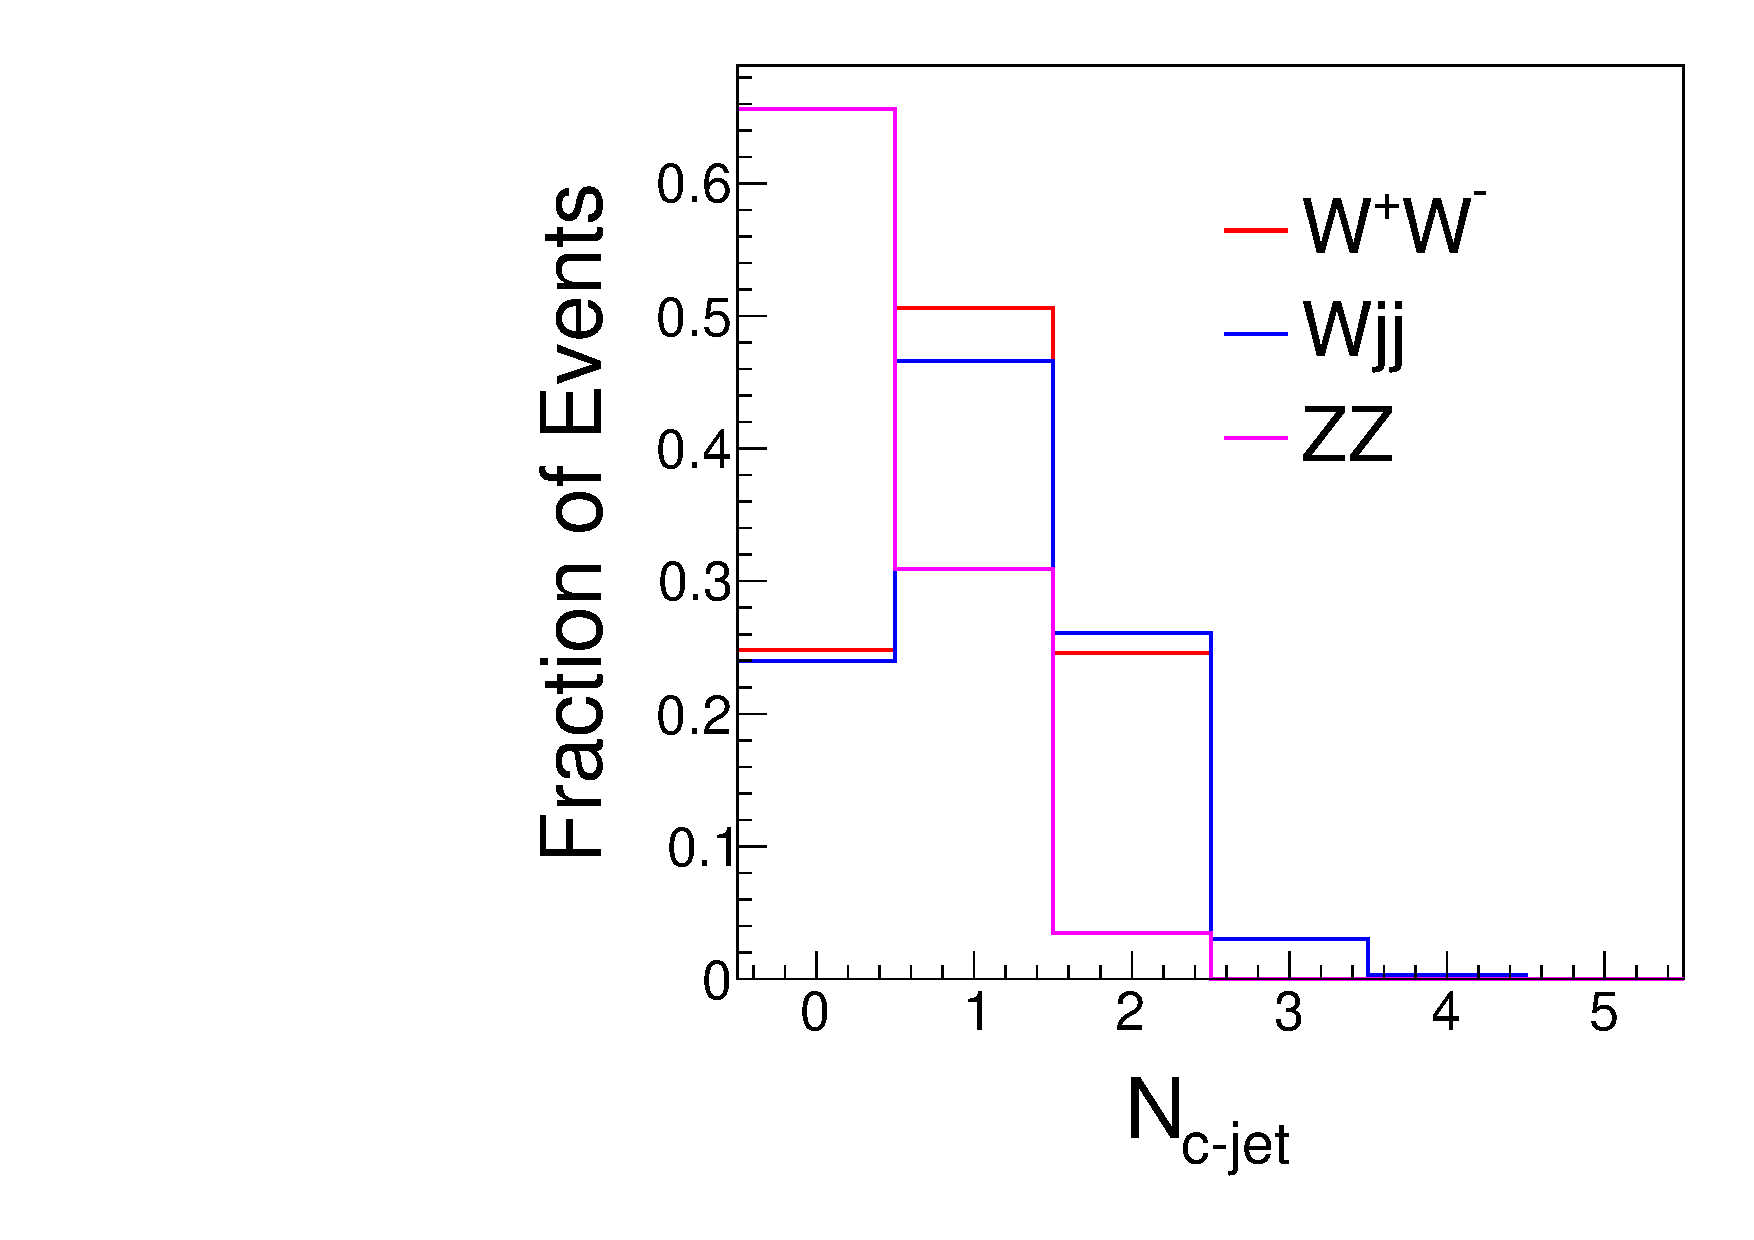
\includegraphics[width=0.4\textwidth]{ncjets_wz.pdf}}
  \caption{The number of (a) true $b$-jets and (b) true $c$-jets in signals and backgrounds with quarks are displayed. As a reference, the number of (c) true $b$-jet and (d) true $c$-jet in background with gauge boson are displayed.}\label{fig:bcjet}
\end{figure}

Below we introduce some simple cuts to separate signal and background events:
\begin{itemize}
  \item Cut1: $N_{jet}=2$, $N_{lepton}=0$ and $M_{jj}>8$ TeV,
  \item Cut2: $150$ GeV$<M(HJ)<200$ GeV,
  \item Cut3: $M(LJ)<75$ GeV,
  \item Cut4: the heavy jet is b-tagged and the light jet is not tagged.
\end{itemize}
The results of the cut flows are listed in Table.~\ref{table:tc:cut}.\xznote{value of benchmark Wilson coefficients?} 
As we can see, the cuts for the invariant masses of heavier and lighter jets are efficient to reduce backgrounds with heavy particles. 
The $b$-tagging cut is efficient to reduce backgrounds with $W$ boson. 
After these cuts, the huge backgrounds are reduced successfully, 
and the signal events can be observed with remarkable significance. 

\begin{center}
\begin{table}
  \begin{center}
  \begin{tabular}{|c|c|c|c|c|c|c|c|}
  \hline
  &  No Cuts  &     Cut1   &  Cut2  & Cut3 & Cut4 &  $S/B$  &    $\sigma$   \\
  \hline
  $\mu^+\mu^-\to tc$   &  2541   & 1168  &  740  &  497 & 304  &  \multirow{8}{*}{0.38} & \multirow{8}{*}{9.12} \\
  $\mu^+\mu^-\to t\bar{t}$     &   $2.15\times{10^4}$  &       $9970$  &  $7602$ & $269$ & $106$  & & \\
  $\mu^+\mu^-\to q\bar{q}$     &   $1.07\times{10^5}$   & $4.93\times{10^4}$  &    $5084$    &  $3498$ & $224$ &   &  \\
  $\mu^+\mu^-\to c\bar{c}$     &   $5.19\times{10^4}$  &  $2.30\times{10^4}$  &    $2365$    &  $1677$ & $210$ &   &  \\
  $\mu^+\mu^-\to b\bar{b}$     &   $2.74\times{10^4}$  & $1.12\times{10^4}$  &    $1158$    &  $829$ & $159$ &   &  \\
  $\mu^+\mu^-\to W^+W^-$  & $7.56\times{10^5}$   & $7.18\times{10^5}$  & $3555$ &  $560$ & $0$ & & \\
  $\mu^+\mu^-\to Wjj$  & $1.07\times{10^6}$  & $3.32\times{10^4}$  &  $2929$   &  $1811$ & $107$  & & \\
  $\mu^+\mu^-\to ZZ$  & $4.55\times{10^4}$   & $4.49\times{10^4}$  &  $0$   &  $0$ & $0$  &  & \\
  \hline
  \end{tabular}
  \end{center}
  \caption{The number of events before and after each cut are listed, where $\sigma$ is defined as $\sigma=S/\sqrt{S+B}$. We assume the luminosity is $30$ ab$^{-1}$ at 10 TeV muon collider. The details of these cuts are described in the text.\label{table:tc:cut}}
\end{table}
\end{center}

For a purpose of comparison and contrast, we also perform an analysis of the process $\mu^+\mu^-\to b\bar{s}(\bar{b}s)$. We introduce the following cuts to separate signal and background events 
\begin{itemize}
  \item Cut1: $N_{jet}=2$, $N_{lepton}=0$, and $M_{jj}>8$ TeV,
  \item Cut2: $M(HJ)<75$ GeV,
  \item Cut3: One jet is b-tagged.
\end{itemize} 
The results of cut flows are listed in Table.~\ref{table:bs:cut}.\xznote{What is the benchmark value for the Wilson coefficients?}

As we discussed above, there should be no massive jets in such signal events, so we can veto the heavier jets by demanding the heavier jet should not have too much larger jet mass.
The jet mass cut of the heavier jets can work to reject backgrounds like $t\bar{t}$, $WW$, and $ZZ$.
The remained backgrounds with $W$ boson can be further reduced by applying a b-tagging cut. After these cuts, it is observed that heavy flavor final states will be the dominant background which leads to a small $S/B$.

\begin{center}
\begin{table}
  \begin{center}
  \begin{tabular}{|c|c|c|c|c|c|c|}
  \hline
  &  No Cuts  &     Cut1 & Cut2 & Cut3 & $S/B$ &  $\sigma$  \\
  \hline
  $\mu^+\mu^-\to bs$     &   4599  &     2080  &  927 & 642   &   \multirow{8}{*}{0.08}   &  \multirow{8}{*}{6.91}  \\
  $\mu^+\mu^-\to t\bar{t}$     &   $2.15\times{10^4}$    & $9970$   &  $2$  & $2$  & & \\
  $\mu^+\mu^-\to q\bar{q}$     &   $1.07\times{10^5}$    &   $4.93\times{10^4}$ & $2.14\times{10^4}$    &  $1066$ &   &  \\
  $\mu^+\mu^-\to c\bar{c}$     &   $5.19\times{10^4}$   &    $2.30\times{10^4}$ & $1.01\times{10^4}$    &  $2207$  &   &  \\
  $\mu^+\mu^-\to b\bar{b}$     &   $2.74\times{10^4}$    &  $1.12\times{10^4}$ &   $4987$    &  $2019$  &   &  \\
  $\mu^+\mu^-\to W^+W^-$  & $7.56\times{10^5}$     &  $7.18\times{10^5}$ &  $1.25\times{10^5}$ &  $1392$ & & \\
  $\mu^+\mu^-\to Wjj$  & $1.07\times{10^6}$   & $3.32\times{10^4}$  &  $1.19\times{10^4}$   &  $1118$  & & \\
  $\mu^+\mu^-\to ZZ$  & $4.55\times{10^4}$  & $4.49\times{10^4}$ &  $447$   &  $188$  &  & \\
  \hline
  \end{tabular}
  \end{center}
  \caption{The number of events before and after each cut is listed. We assume the luminosity is $30$ ab$^{-1}$ at 10 TeV muon collider. The details of these cuts are described in the text.\label{table:bs:cut}}
\end{table}
\end{center}

Fig.~\ref{fig:cll1d} shows the $2\sigma$ and $3\sigma$ bounds on the $C^{X}_{LL}$.

\begin{figure}[htbp]
  \setcounter{subfigure}{0}
  \centering
  % Requires \usepackage{graphicx}
  \subfigure{
  \thesubfigure
  \label{fig:clltc1d}
  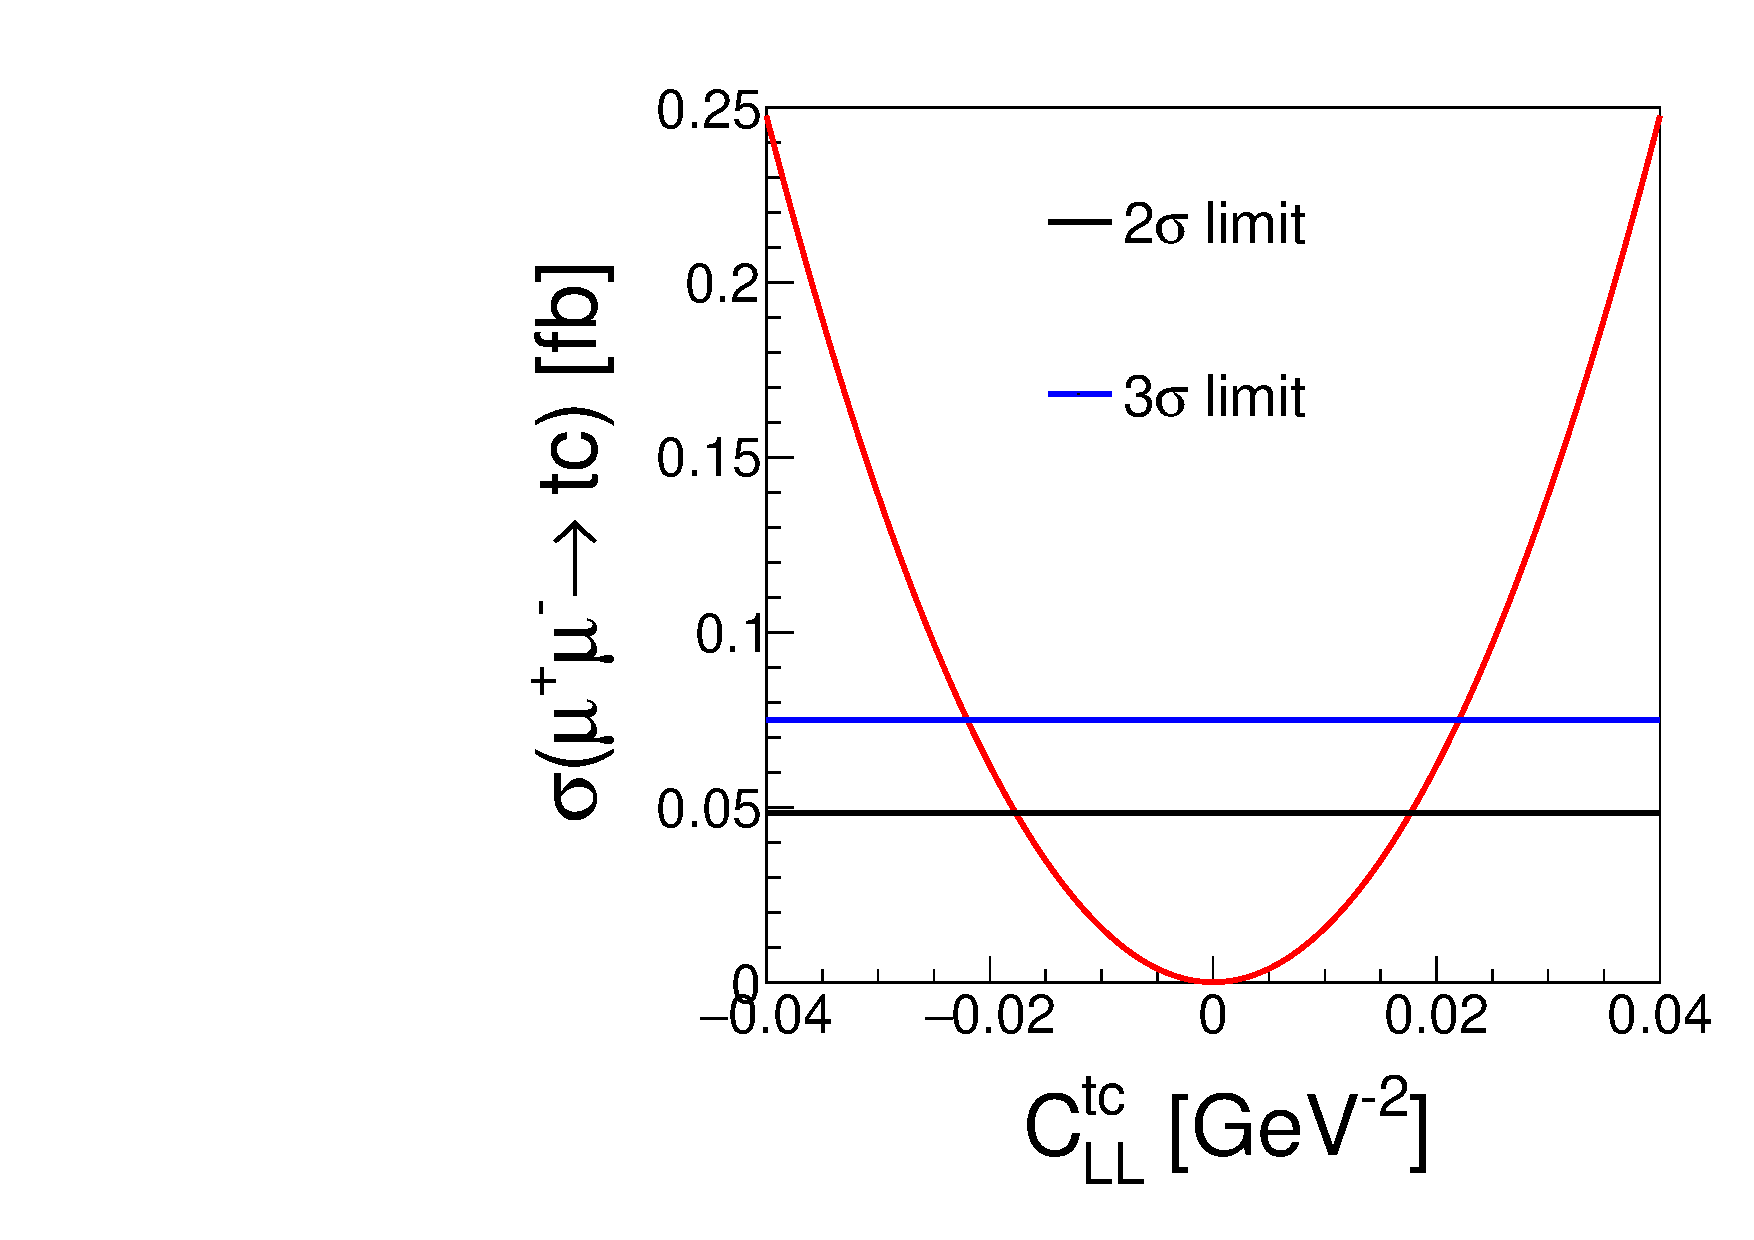
\includegraphics[width=0.4\textwidth]{clltc1d.pdf}}
  \subfigure{
  \thesubfigure
  \label{fig:cllbs1d}
  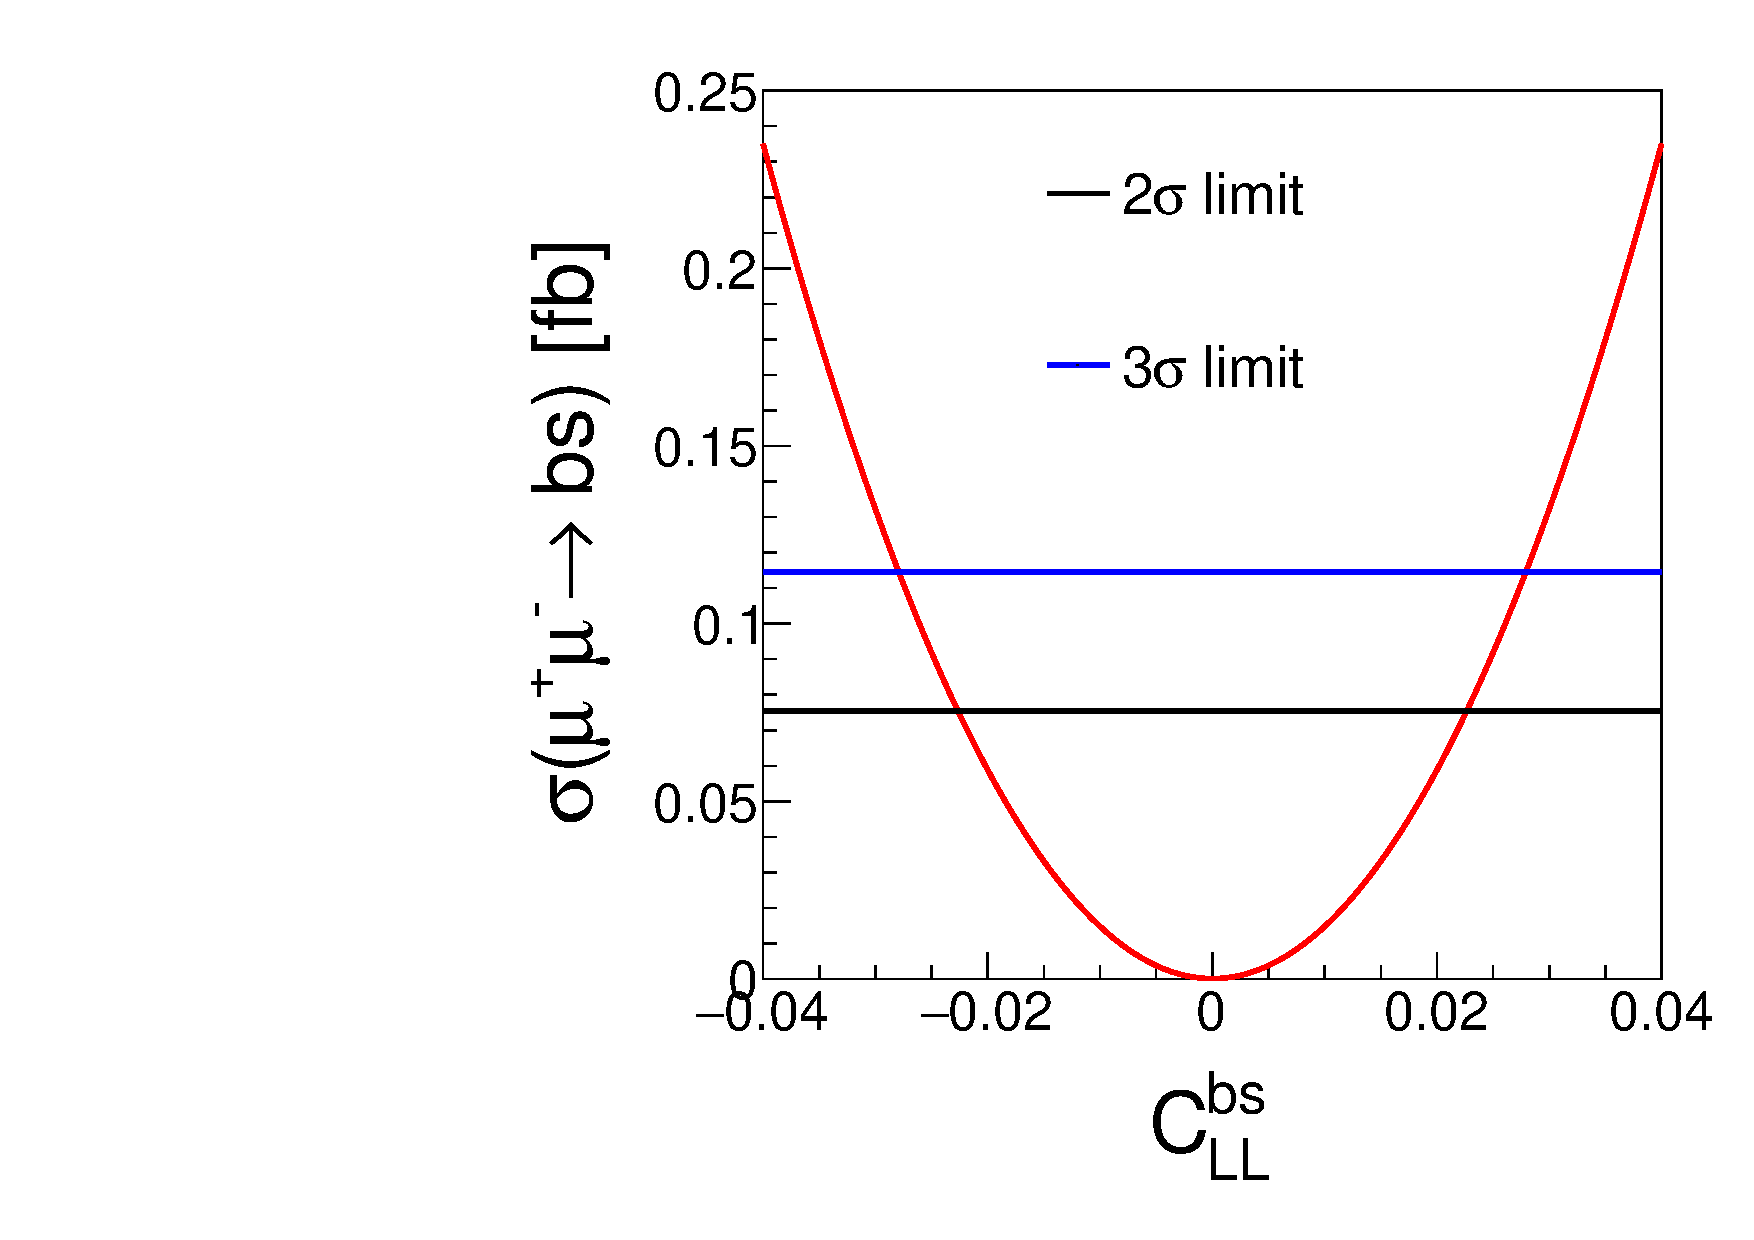
\includegraphics[width=0.4\textwidth]{cllbs1d.pdf}}
  \caption{The $2\sigma$ and $3\sigma$ bounds of (a) $C^{tc}_{LL}$ and (b) $C^{bs}_{LL}$ at 10 TeV muon collider with luminosity $\mathcal{L}=10$ ab$^{-1}$.}\label{fig:cll1d}
\end{figure}

\begin{figure}
    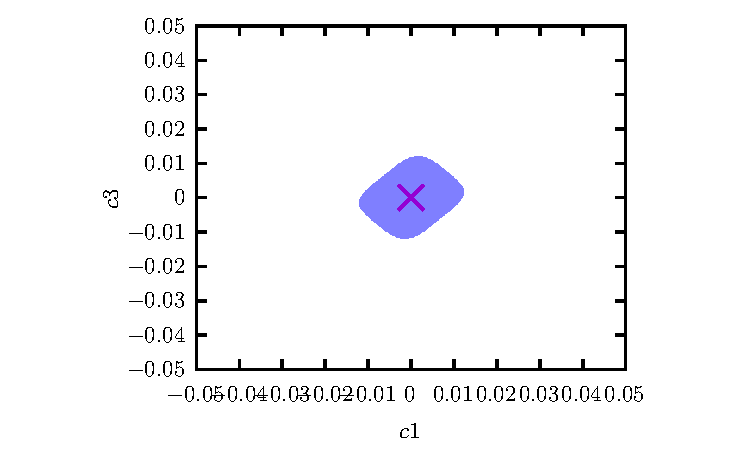
\includegraphics[width=0.4\textwidth]{2dbound.pdf}
    \caption{The $2\sigma$ bounds are shown.\xznote{Currently using 0.03 as reference value, need to be updated.}}\label{fig:cll2d}
\end{figure}

\section{Summary and Discussion}\label{Sec:conc}
For the signal processes $\mu^+ \mu^- \to b s$ \cite{Altmannshofer:2022xri}, it has been revealed that b tagging is crucial to reject background events from $jj$ final states. The dominant background events are $j j$. In order to extract the information on the Wilson coefficients $C_{9}$ and $C_{10}$, it is found that the polarized muon beams and the measurement of forward-backward asymmetry of the final state are needed. 

In this work, instead of assuming polarized muon beams and charge tagging of a final state, we propose to measure the signal processes $\mu^+ \mu^- \to t c$. Then it is found that the major task is to reject $t \bar{t}$ and $ W W$ events, which might be easier to pick out signal events. It is also found that the weak radiation $ j j W$ is large and might be a relevant background.

It is also found that in order to resolve the signal events, detectors with high granularity are needed since top quarks and W bosons in the hadronic final states are around 5 TeV and are highly boosted objects. In order to capture the substructure of these massive jets, the cone parameter should be set as around  $0.09-0.1$ when the collision energy is assumed to be $\sqrt{s}=10$ TeV, which is much smaller compared with the cone parameter adopted as $R=0.4$ or $0.5$ at the LHC. To extract signal events from large background events, a refined analysis of the jet substructure at TeV region should be applied in order to achieve much better performance. \textcolor{black}{It is expected that a modern top tagger technique can improve the top jet identification and reject the W/Z jets.}


To distinguish new physics models, it is found that the measurement of  $\mu^+ \mu^- \to tc$ can pinpoint Model I and Model II. Model III can be discovered due to the resonance near a few TeV regions. Model IV could be favored if there is no signal of the process $\mu^+ \mu^- \to t c$ are measured.

	\begin{acknowledgments}
                Z.J. Zhao has been partially supported by a
		Nikolai Uraltsev Fellowship of the Center for Particle Physics,
		University of Siegen, and partially supported by the Natural Science
		Foundation of China under the grant No. 11875260. 
		S.C. Sun is supported by the National Natural Science Foundation of China, No.12105013.
		Q.S. Yan is supported by the Natural Science Foundation of China
		under the grant No.  11475180 and No. 11875260.
		X.R. Zhao is supported by the Italian Ministry of Research (MUR) under grand PRIN 20172LNEEZ.

	\end{acknowledgments}

\appendix
	



\section{SMEFT Renormalization Group Equation}\label{smeftrge}
The RGE of SMEFT Wilson coefficients can be written as 
\begin{eqnarray}
  \frac{dC_i}{d\ln{\mu}} &=& \frac{1}{16\pi^2}\beta_i. \label{beta:definition}
\end{eqnarray}
All 1-loop $\beta$ functions of operators in Warsaw basis have been derived in Ref.~\cite{Celis:2017hod}. 

The $\beta$ functions of operators~\ref{O1lq}$\sim$\ref{Oqe} are
\begin{eqnarray}
   \left[\beta^{(1)}_{lq}\right]_{prst} &=& \frac{2}{3}{g^\prime}^2\left([C^{(1)}_{lq}]_{wwst}+[C_{qe}]_{stww}\right)\delta_{pr}-{g^\prime}^2[C^{(1)}_{lq}]_{prst}  \nonumber \\
   &&+9g^2[C^{(3)}_{lq}]_{prst}+\frac{1}{2}[\Gamma_u^\dagger\Gamma_u]_{vt}[C^{(1)}_{lq}]_{prsv}, \label{beta:lq1}  \\
   \left[\beta^{(3)}_{lq}\right]_{prst} &=& \frac{2}{3}g^2[C^{(3)}_{lq}]_{wwst}\delta_{pr}+3g^2[C^{(1)}_{lq}]_{prst}-(6g^2+{g^\prime}^2)[C^{(3)}_{lq}]_{prst}  \nonumber \\ 
   && +\frac{1}{2}[\Gamma_u^\dagger\Gamma_u]_{vt}[C^{(3)}_{lq}]_{prsv}, \label{beta:lq3} \\
   \left[\beta_{qe}\right]_{prst} &=& \frac{4}{3}{g^{\prime}}^2\left([C^{(1)}_{lq}]_{wwpr}+[C_{qe}]_{prww}\right)\delta_{st}+2{g^{\prime}}^2[C_{qe}]_{prst} \nonumber  \\
   && +\frac{1}{2}[\Gamma_u^\dagger\Gamma_u]_{vr}[C^{(1)}_{lq}]_{pvst}, \label{beta:qe}
\end{eqnarray}
where $g$ and $g^\prime$ are the gauge coupling of $SU(2)$ and $U(1)$, respectively. 
$\Gamma_{u}$ is the $3\times 3$ Yukawa mass matrix of u-type quarks. 
For simplicity, we only consider the top quark is massive, 
and only the element $\Gamma_u(3,3)=1$ is non-zero.
Note the Eq.~\ref{beta:lq1}$\sim$\ref{beta:qe} only contains the most important contributions and mixing of the corresponding operators. 
The mixing of the full set of operators is beyond the scope of this work. 

The 1-loop RGE running of SM parameters is given by these $\beta$ functions:
\begin{eqnarray}
  \beta_{g} &=& -\frac{19}{6}g^3,  \\
  \beta_{g^\prime} &=& \frac{41}{6}{g^\prime}^3,  \\
  \beta_{g_s} &=& -7g^2_s, \\
  \left[\beta_{\Gamma_u}\right]_{33} &=& \frac{9}{4}g^2\Gamma_u(3,3)-\frac{17}{12} {g^\prime}^2\Gamma_u(3,3)-8g^2_s\Gamma_u(3,3)+\frac{9}{2}\Gamma^3_u(3,3).
\end{eqnarray}

Our simplified RGE running has been compared with two tools: DSixTools~\cite{Celis:2017hod,Fuentes-Martin:2020zaz} and Wilson~\cite{Aebischer:2018bkb}.
The differences between our results and these tools are below $1\%$.


\section{LEFT Renormalization Group Equation}\label{leftrge}

The definition of RGE of LEFT is the same as Eq.~\ref{beta:definition}, but $C_i$ are replaced by $L_i$.
The $\beta$ functions of operator~\ref{QVLLed} and \ref{QVLRde} are
\begin{eqnarray}
  \left[\beta^{V,LL}_{ed}\right]_{prst} &=& \frac{4}{3}e^2q_eq_d\delta_{pr}\left([L^{V,LL}_{ed}]_{wwst}+[L^{V,LL}_{ed}]_{stww}\right)+12e^2q_eq_d[L^{V,LL}_{ed}]_{prst},  \label{beta:VLLed} \\
  \left[\beta^{V,LR}_{de}\right]_{prst} &=& \frac{4}{3}e^2q^2_e\delta_{st}\left([L^{V,LL}_{ed}]_{wwpr}+[L^{V,LR}_{de}]_{prww}\right)-12e^2q_eq_d[L^{V,LR}_{de}]_{prst}, \label{beta:VLRde}
\end{eqnarray}
where $e$ is the coupling constant of QED. 
$q_e=-1$ and $q_d=-1/3$ are the charges of lepton and d-type quark, respectively. 

At the low energy scale, the 1-loop running of QCD and QED coupling is given by the following $\beta$ functions:
\begin{eqnarray}
  \beta_{g_s} &=& -\frac{23}{3}g^3_s,  \\
  \beta_{e} &=& \frac{80}{9}e^3, 
\end{eqnarray}







		\bibliographystyle{JHEP}
		\bibliography{eetc}

		\end{document}

